%\documentclass[a4paper,twoside]{article}
\documentclass[12pt]{extarticle}

\usepackage[margin=2cm]{geometry}


\usepackage[utf8x]{inputenc}
%\usepackage[cp1251]{inputenc}
\usepackage[T2A]{fontenc}
\usepackage{array}
\usepackage{amssymb}
\usepackage{amsmath}
\usepackage{amsthm}
\usepackage{latexsym}
\usepackage{indentfirst}
\usepackage{bm}
\usepackage{enumerate}
\usepackage{graphicx}
\usepackage{epsf}
%\usepackage{epsfig}
%\DeclareGraphicsExtensions{.pdf,.png,.jpg}
\usepackage{wrapfig}
\usepackage{euscript}
\usepackage{indentfirst}
\usepackage[english,russian]{babel}
\usepackage{microtype}
% \sloppy\unitlength=.24mm
% \renewcommand{\thefootnote}{\arabic{footnote}}

% \textwidth=132mm
% \headheight=7mm
% \headsep=5mm
% \textheight=200mm
% \oddsidemargin=0mm
% \evensidemargin=0mm
% \topmargin=0mm

\newcommand{\firstheader}[1]{\noindent\textbf{#1}\nopagebreak\bigskip}
\newcommand{\header}[1]{\bigskip\medskip\noindent\textbf{#1}\nopagebreak\bigskip}
\newcommand{\subheader}[1]{\bigskip\medskip\noindent\emph{#1}\nopagebreak\bigskip}
\newcommand{\subsub}[1]{\bigskip\medskip\noindent\emph{#1}\nopagebreak\bigskip}

\theoremstyle{theorem}
\newtheorem{theorem}{Теорема}
\newtheorem{Theorem}{Теорема}
\newtheorem{definition}{Определение}
\newtheorem{Def}{Определение}
\newtheorem{corollary}{Следствие}
\newtheorem{proposition}{Предложение}
\newtheorem{prop}{Предположение}
\newtheorem{lemma}{Лемма}
\newtheorem{assumption}{Предположение}
\newtheorem{Lemma}{Лемма}
\newtheorem{Cons}{Следствие}
\newtheorem{Proposition}{Предложение}
\newtheorem{Statement}{Утверждение}
\newtheorem{statement}{Утверждение}
\theoremstyle{remark}
\newtheorem{remark}{Замечание}
\newtheorem{Remark}{Замечание}
\newtheorem{example}{Пример}
\newtheorem{Example}{Пример}
\newtheorem{notation}{Замечание}
\newtheorem{teo}{Теорема}
\newtheorem{sled}{Следствие}
\newtheorem{sublemma}[theorem]{\indent\bf Подлемма}
\newtheorem{problem}{\indent\bf Проблема}
\newtheorem{hypothesis}{\indent\bf Гипотеза}
\newtheorem{denotation}[theorem]{\indent\bf Обозначение}
\newtheorem{thr}{Теорема}
\newtheorem{crl}[thr]{Следствие}
\newtheorem{lmm}[thr]{Лемма}
\newtheorem{qu}{Вопрос}
\newtheorem{dfn}{Определение}
\newtheorem{approval}{Утверждение}

\makeatletter
\renewcommand*{\hm}[1]{#1\nobreak\discretionary{}%
	{\hbox{$\mathsurround=0pt #1$}}{}}% перенос арифметических знаков
\newcommand{\rmnum}[1]{\romannumeral #1}
\newcommand{\Rmnum}[1]{\expandafter\@slowromancap\romannumeral #1@}
\usepackage{lipsum}
\newcommand{\Mark}{\{(\Gamma_i, \varkappa_i); \hm{} i \geqslant 0\}}
\renewcommand{\Pr}{{\mathbf P}}
\newcommand{\No}{\textnumero}
\usepackage[noadjust]{cite}

% нумерацию можно оставить как есть
\newcommand{\pages}{1-8}

\begin{document}

\begin{titlepage}

  \begin{center}
  \textls[-80]{
    \textbf{МИНИСТЕРСТВО ОБРАЗОВАНИЯ И НАУКИ РОССИЙСКОЙ ФЕДЕРАЦИИ} }\\
    \textls[-30]{
    \textbf{%
    {ФГАОУ ВО 
      <<Нижегородский государственный университет им.~Н.И.~Лобачевского>>}
    }
    }

 \medskip

 
   \textbf{ Институт информационных технологий, математики и механики }\\
    Кафедра математического обеспечения и суперкомпьютерных технологий

    
 \medskip
  \medskip
   \medskip \medskip
    \medskip
     \medskip
      \medskip
     \hfill
    \begin{minipage}[h]{ 0.31\linewidth}
    <<УТВЕРЖДАЮ>>\\
    Руководитель \\
    исследовательской практики\\
\\
    \underline{\hspace{3cm}} Зорин~А.В.
    \end{minipage}
   \medskip \medskip
    \medskip
     \medskip
      \medskip
   \medskip \medskip
    \medskip
     \medskip
      \medskip
      
    \textbf{ОТЧЕТ  ПО}\\ \textbf{ИССЛЕДОВАТЕЛЬСКОЙ ПРАКТИКЕ}\\
 \medskip
    \textbf{по теме:} \\
    <<Достаточное условие существования стационарного режима очередей \\ первичных требований в тандеме систем массового обслуживания>>
    
         \medskip
      \medskip
               \medskip
      \medskip
    \hfill
    \begin{minipage}[h]{ 0.5\linewidth}
    Аспиранта 4 года обучения\\
    Кочеганова В.М.
    \end{minipage}
    \vfill {Н.Новгород, 2018}
  \end{center}
\end{titlepage}


\tableofcontents
\newpage

\section{Информация об исследовательской практике}
\begin{enumerate}
    \item Сроки прохождения исследовательской практики: с 02.10.2017 по 31.01.2018.
    \item База исследовательской практики: кафедра программной инженерии, \newline Нижегородский государственный университет им.~Н.И.~Лобачевского, \newline {г.~Нижний Новгород}
\end{enumerate}
\newpage
\section{Введение}

В связи со стремительным ростом числа машин в современных городах все больший интерес стала представлять теория потоков транспортных средств. Результаты ранних исследований по этой тематике собраны, например, в книгах \cite{Haight:1963, Drew:1968, Inose:1975}. В этих монографиях потоки машин моделируются с помощью традиционных стохастических потоков событий, весьма полно изученных в классической теории массового обслуживания. Однако классические модели не удается использовать для адекватного описания реальных потоков машин (см. \cite{Bartlet:1963, Cox:1969,Dshalalov:1997}). В работах
\cite{Fedotkin:Kudryavcev:Rachinskaya:2010, Rachinskaya:Fedotkin:2011:1, Rachinskaya:Fedotkin:2014} предлагается учитывать не только вероятностные свойства последовательности моментов пересечения машинами так называемой виртуальной стоп-линии, но и определять свойства случайных конфигураций автомобилей на дороге. В указанных работах изучается возникновение так называемых пачек машин. Каждая пачка состоит из медленной головной машины и ожидающих возможности обгона машин за ней. Динамика длины пачки определяется возможностью обгона машинами из хвоста всей пачки. Другая динамика, обусловленная возможностью съезда машин с трассы, рассматривается в работах \cite{Afanasyeva:Bulinskaya:2013:1,Afanasyeva:Bulinskaya:2010,Afanasyeva:Bulinskaya:2013:2}. Основным объектом изучения в этих работах является плотность потока машин как функция от расстояния, а знание плотности, в свою очередь, позволяет делать выводы о пропускной способности перекрестков.

Тандемы систем массового обслуживания широко используются при моделировании компьютерных и коммуникационных систем, колл-центров, аварийных служб, при планировании их мощностей, производительности и последующей оптимизации работы. 
Тандем является простейшей сетью из нескольких приборов, в которой заявка после обслуживания на одном устройстве  поступает в очередь на обслуживание следующим устройством.
Одной из первых работ, посвященная тандемам систем массового обслуживания, является работа \cite{Reich:1957}. В ней изучается распределение времени пребывания требования в системе с двумя обслуживающими устройствами. В предположении, что промежутки времени между поступлением заявок в систему и времени обслуживания независимы и имею экпоненциальные законы распределения, было показано, что время ожидания требования в очереди первого прибора стохастически не зависит от его времени ожидания в очереди второго прибора. 

Основные результаты теории тандемов в случае простейших стационарных входных потоков и экспоненциального времени обслуживания широко представлены, например, в работах \cite{Balsamo:2003, Gnedenko:Konig:1983, Perros:1994}. Модели с неэкспоненциальным временем обслуживания рассмотрены в статьях \cite{Gomez:2002:1, Gomez:2002:2, Gomez:2002:3}. Более общие модели включают в себя так называемые входные BMAP (Batch Markovian Arrival Process) потоки, особенностью которых является наличие корреляции количества пришедших требований в различные моменты времени. Системы обслуживания с входными потоками типа BMAP рассмотрены, например, в работах \cite{Klimenok:Dudin:2005, Klimenok:2010, Klimenok:2015}, где проведены аналитические рассчеты условий стационарности и изучено поведение характеристик обслуживания для двухфазных (тандемных) систем, в том числе с повторными попытками и нетерпеливыми требованиями. 
Модель последовательных перекрестков с немгновенным перемещением машин между ними была впервые предложена в работах \cite{Zorine:2012,Zorine:2013}. В этих работах динамика перемещения машин от одного перекрестка к другому задается бернулиевской случайной величиной: каждая машина с некоторой фиксированной вероятностью $0<p<1$ успевает доехать до следующего перекрестка и с противоположной вероятностью $1-p$ остается <<между>> перекрестками.

Cтатья \cite{Kocheganov:2017:1} отличается от работ  \cite{Zorine:2012,Zorine:2013} введением продления в алгоритм обслуживания во второй системе. 
В данной работе рассматривается тандем из двух систем массового обслуживания. В первой системе управление осуществляется по циклическому алгоритму. После обслуживания в первой системе, требования немгновенно поступают на вторую, где обслуживаются по циклическому алгоритму с продлением. Целью этой статьи является исследование условий существования стационарного режима очередей первичных требований, то есть требований, генерируемых внешней средой.

\section{Постановка задачи на содержательном уровне}

Рассмотрим систему массового обслуживания следующего вида (рис.~\ref{SystemScheme}).
\begin{figure}[h]
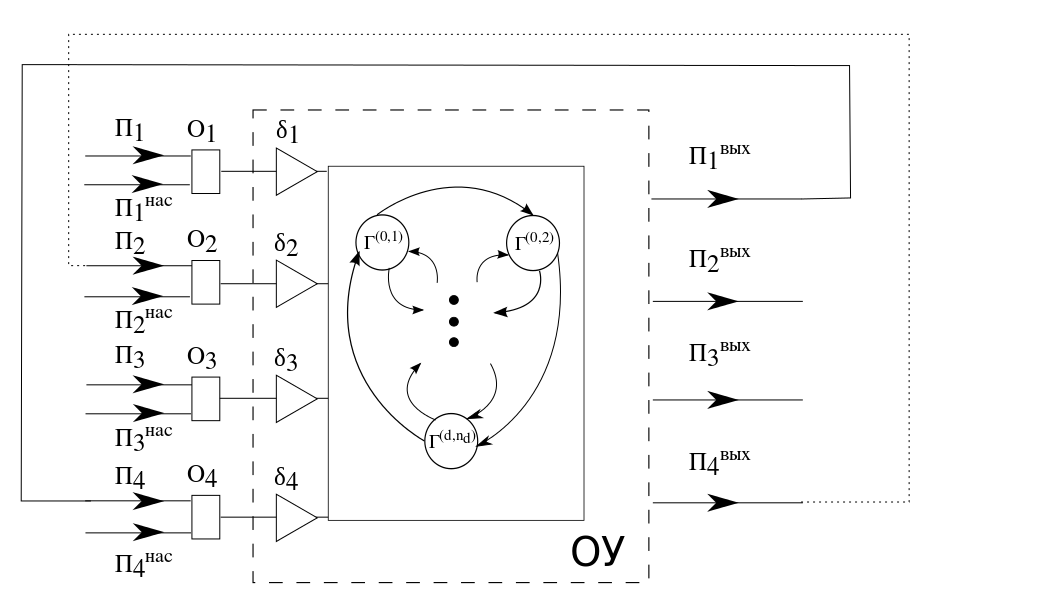
\includegraphics[scale=0.4]{SystemScheme.png} 
\caption{Структурная схема системы обслуживания}
\label{SystemScheme}
\end{figure}
Пусть в систему с одним обслуживающим устройством поступают потоки $\Pi_1$, $\Pi_2$, $\Pi_3$  и $\Pi_4$. Требования по потоку $\Pi_j$ становятся в соответствующую очередь $O_j$ с неограниченной вместимостью, $j\in \{1, 2, 3, 4\}$. Для $j \in \{1, 2, 3\}$ дисциплина очереди $O_j$, поддерживаемая устройством $\delta_j$, имеет тип FIFO (First In First Out). Таким образом, для обслуживания из соответствующей очереди выбирается то требование, которое пришло раньше. Дисциплина очереди $O_4$ будет описана ниже. Входные потоки $\Pi_1$ и $\Pi_3$ формируются внешней средой, которая, будем предполагать, имеет только одно состояние, то есть вероятностная структура потоков не меняется с течением времени. Требования потоков $\Pi_1$ и $\Pi_3$ формируют независимые между собой неординарные пуассоновские потоки, то есть  стационарные, без последействия и ординарные потоки групп требований. Интенсивности соответствующих простейших потоков для $\Pi_1$ и $\Pi_3$ будем обозначать $\lambda_1$ и $\lambda_3$, а распределение числа заявок в группе по потоку $\Pi_j$ будем описывать производящей функцией
\begin{equation}
f_j(z) = \sum_{\nu=1}^{\infty} p_{\nu}^{(j)} z ^{\nu}, \quad j\in \{1,3\},
\label{GeneratingFunc}
\end{equation}
которая предполагается аналитической при любом $z\in \mathbb{C}$ таком, что $|z|<(1+\varepsilon)$, $\varepsilon>0$. Величина $p_{\nu}^{(j)}$ определяет вероятность того, что по потоку $\Pi_j$ число требований в группе равно $\nu$. Обслуженные требования потока $\Pi_1$ поступают на повторное обслуживание, формируя на выходе поток $\Pi_4$. Обслуженные требования потока $\Pi_4$ в свою очередь поступают на повторное обслуживание, формируя при этом поток $\Pi_2$. Потоки $\Pi_2$ и $\Pi_3$ являются конфликтными, что означает запрет на одновременное обслуживание требований этих потоков и, следовательно, исследование системы не может быть сведено к задаче с меньшим числом потоков. 

В каждый момент времени обслуживающее устройство находится в одном из конечного множества состояний $\Gamma=\{\Gamma^{(k,r)} \colon k=\overline{0,d}; r=\overline{1,n_k}\}$ с заданными натуральными числами $d$, $n_0$, $n_1$, $\ldots$, $n_d$. В каждом состоянии $\Gamma^{(k,r)}$ обслуживающее устройство находится в течение неслучайного времени $T^{(k,r)}$. 
Введем непересекающиеся подмножества $\Gamma^{\mathrm{I}}$, $\Gamma^{\mathrm{II}}$, $\Gamma^{\mathrm{III}}$ и $\Gamma^{\mathrm{IV}}$ множества $\Gamma$ следующим образом. 
В состоянии $\Gamma^{(k,r)} \in \Gamma^{\mathrm{\Rmnum{1}}}$ обслуживаются только требования из очередей $O_1$, $O_2$ и $O_4$.
В состоянии $\gamma \in \Gamma^{\mathrm{\Rmnum{2}}}$ обслуживаются только требования из очередей $O_2$ и $O_4$.
В состоянии $\gamma \in \Gamma^{\mathrm{\Rmnum{3}}}$ обслуживаются только требования из очередей $O_1$, $O_3$ и $O_4$.
В состоянии $\gamma \in \Gamma^{\mathrm{\Rmnum{4}}}$ обслуживаются только требования из очередей $O_3$ и $O_4$.
Тогда множество $\Gamma$ есть объединение $\Gamma = \Gamma^{\mathrm{I}} \cup \Gamma^{\mathrm{II}} \cup \Gamma^{\mathrm{III}} \cup \Gamma^{\mathrm{III}}$ непересекающихся подмножеств. Также в дальнейшем нам понадобятся множества ${}^1\Gamma=\Gamma^{\mathrm{\Rmnum{1}}} \cup \Gamma^{\mathrm{\Rmnum{3}}}$, 
${}^2\Gamma=\Gamma^{\mathrm{\Rmnum{1}}} \cup \Gamma^{\mathrm{\Rmnum{2}}}$,
${}^3\Gamma=\Gamma^{\mathrm{\Rmnum{3}}} \cup \Gamma^{\mathrm{\Rmnum{4}}}$. 

\begin{figure}[t]\centering
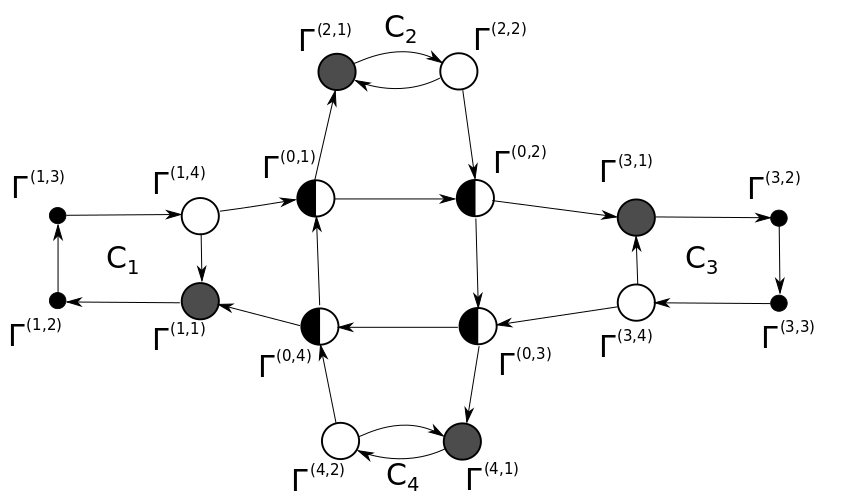
\includegraphics[scale=0.44]{GraphScheme3_grayscale.png} 
\caption{Класс графов переходов. Незакрашенные вершины являются выходными вершинами, большие черные вершины --- входные, небольшие черные --- нейтральные, наполовину закрашенным вершинам соответствуют состояния продления}
\label{GraphScheme}
\end{figure}

Смена состояний обслуживающего устройства осуществляется по следующему правилу. Множество состояний $C_k = \{\Gamma^{(k,r)} \colon r=\overline{1,n_k}\}$ будем называть $k$-м циклом, $k=\overline{1,d}$ (Рис. \ref{GraphScheme}). Состояние вида $\Gamma^{(0,r)}$ будем называть состоянием продления, $r=\overline{1,n_0}$. Положим $r \oplus_k 1 = r+1$ для $r=\overline{1,n_k-1}$ и $r \oplus_k 1 = 1$ при $r=n_k$, $k = \overline{0,d}$. В цикле $C_k$ выделим подмножества $C_k^{\mathrm{O}}$ выходных, $C_k^{\mathrm{I}}$ входных и $C_k^{\mathrm{N}} = C_k \setminus (C_k^{\mathrm{O}} \cup C_k^{\mathrm{I}})$ нейтральных состояний. Тогда после состояния $\Gamma^{(k,r)} \hm\in C_k\setminus C_k^{\mathrm{O}}$ обслуживающее устройство переходит в состояние $\Gamma^{(k,r \oplus_k 1)}$ того же цикла $C_k$. При $\Gamma^{(k,r)}$ принадлежащем множеству $C_k^{\mathrm{O}}$ прибор переходит в состояние $\Gamma^{(k,r \oplus_k 1)}$, если число требований в очереди $O_3$ в момент переключения больше заданного порога $L$. В противном случае, то есть если число требований в очереди $O_3$ меньше либо равно $L$, новое состояние прибора будет состоянием продления $\Gamma^{(0,r_1)}$, где $r_1=h_1(\Gamma^{(k,r)})$ и $h_1(\cdot)$~--- заданное отображение множества $\bigcup\limits_{k=1}^d C_k^{\mathrm{O}}$ во множество $\{1,2,\ldots, n_0\}$. После состояния $\Gamma^{(0,r)}$ выбирается состояние того же вида $\Gamma^{(0,r_2)}$, если число требований в очереди $O_3$ меньше или равно $L$, где $r_2=h_2(r)$ и $h_2(\cdot)$~--- заданное отображение множества $\{1,2, \ldots, n_0\}$ на себя; в противном случае включается входное состояние $\Gamma^{(k,r_3)} \in C_k^{\mathrm{I}}$, где $\Gamma^{(k,r_3)}=h_3(r)$ и $h_3(\cdot)$~--- заданное отображение множества $\{1,2, \ldots, n_0\}$ на множество  $\bigcup\limits_{k=1}^d C_k^{\mathrm{I}}$. Считается, что все состояния продления $\Gamma^{(0,r)}$ принадлежат множеству ${}^2 \Gamma$, а также верны соотношения $C_k^\mathrm{O}\subset {}^2 \Gamma$ и $C_k^\mathrm{I}\subset {}^3 \Gamma$. Также будем предполагать, что все циклы имеют ровно одно входное и одно выходное состояние. И последним предположением является то, что все вершины продления образуют один цикл, то есть можем положить $h_2(r)=r\oplus_0 1$.


%\subsection{Допустимые графы переходов состояний ОУ}

Таким образом, смена состояний обслуживающего устройства задается соотношением:
\begin{equation}
h(\Gamma^{(k,r)},y) = 
\begin{cases}
\Gamma^{(k,r \oplus_k 1)},&  \text{если } (\Gamma^{(k,r)}\in C_k\setminus C_k^{\mathrm{O}}) \text{ или } (\Gamma^{(k,r)}\in C_k^{\mathrm{O}} \text{ \& } y>L);\\
%\Gamma^{(k,r \oplus_k 1)},& \quad \text{ если } \Gamma^{(k,r)}\in C_k^{\mathrm{O}} \text{ и } y>L;\\
\Gamma^{(0,h_1(\Gamma^{(k,r)}))},&  \text{если } \Gamma^{(k,r)}\in C_k^{\mathrm{O}} \text{ и } y\leqslant L;\\
\Gamma^{(0,r \oplus_0 1)},&  \text{если } k=0 \text{ и } y\leqslant L;\\
h_3(r),&  \text{если } k=0 \text{ и } y > L.
\end{cases}
\label{hLaw}
\end{equation}

В качестве наглядной физической интерпретации можно привести тандем из двух перекрестков (рис. \ref{crossroads}).
\begin{figure}[t]
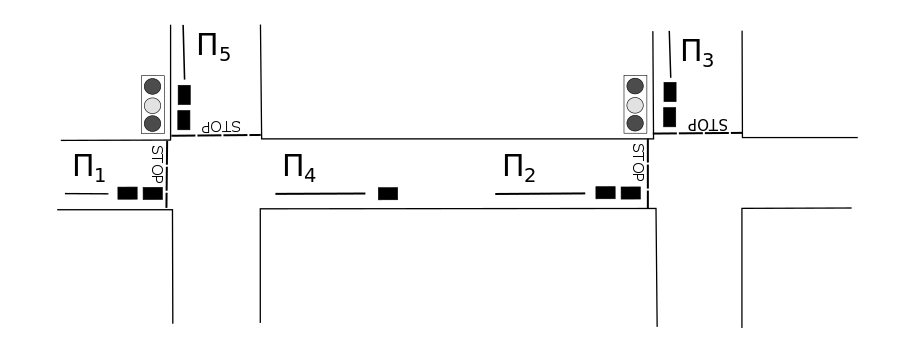
\includegraphics[scale=0.41]{Crossroads_grayscale.png}
\caption{Пример: тандем перекрестков}
\label{crossroads}
\end{figure}
В роли потоков требований, формируемых внешней средой, выступают потоки прибывающих на перекрестки машин: конфликтные потоки $\Pi_1$, $\Pi_5$ на первом перекрестке, а также поток $\Pi_3$ на втором. Каждая машина из потока $\Pi_1$, проезжая первый перекресток, становится в очередь $O_4$ потока $\Pi_4$ и затем с некой вероятностью ($p_{k,r}$ для состояния $\Gamma^{(k,r)}$ обслуживающего устройства) доезжает до следующего перекрестка, или же не успевает это сделать и остается в очереди $O_4$ до следующего такта обслуживания. В случае, если машина из очереди $O_4$ успевает доехать до второго перекрестка, она становится в очередь $O_2$ и ждет своей очереди для его прохождения.

Предполагается, что светофор на первом перекрестке имеет лишь два состояния $\{g_{1,1},g_{1,2}\}$: в состоянии $g_{1,1}$ машины потока $\Pi_1$ пропускаются фиксированное количество времени $\widetilde T^{(1,1)}$ (<<зеленый>> свет для $\Pi_1$); в состоянии $g_{1,2}$ --- простаивают в течение времени $\widetilde T^{(1,2)}$ (<<красный>> свет для $\Pi_1$). Светофор на втором перекрестке обслуживает по алгоритму с продлением: дополнительно к состоянию обслуживания потока $\Pi_3$ (состояние $g_{2,1}$), также имеется два состояния обслуживания потока $\Pi_2$ (состояния $\{g_{2,2},g_{2,3}\}$). Первое из них включается всегда после завершения обслуживания потока $\Pi_3$, а второе включается, если после очередного такта обслуживания потока $\Pi_2$ длина очереди $O_3$ не превосходит уровня $L$.
Длительности пребывания светофора на втором перекрестке в каждом из состояний суть $\widetilde T^{(2,1)}$, $\widetilde T^{(2,2)}$ и $\widetilde T^{(2,3)}$.


Рассматривая тандем из двух перекрестков как единую систему массового обслуживания и предполагая наблюдение за ней только в (дискретные) моменты переключения состояния хотя бы одного из светофоров, можно показать, что количество различных состояний у полученной системы конечно. Действительно, положим, например, за состояние объединенной системы вектор $(g^{(1)},g^{(2)}, s, t)$, где $g^{(1)}\in \{g_{1,1},g_{1,2}\}$~--- состояние $1$--го перекрестка, $g^{(2)}\in \{g_{2,1},g_{2,2},g_{2,3}\}$~--- состояние $2$--го перекрестка, $s \in \{0, 1, 2\}$~--- номер последнего сменившего состояние перекрестка (принимает значение $0$ в случае, если сменили состояние оба перекрестка) и $t \in \{0, 1, 2, \ldots, T\}$~--- количество времени, оставшееся у продолжающего обслуживание с прошлого такта перекрестка (принимает значение $0$, если принимает значение $0$ величина $s$). Здесь $T$~--- максимальная длительность нахождения каждого из светофоров в одном состоянии. Тогда количество различных состояний не трудно посчитать и оно не будет превышать величины  $2\times 3 \times 3 \times T$.

В завершение построения примера отметим, что при прохождении перекрестков машины предполагаются движущимися только в прямом направлении, то есть перемешивания конфликтных потоков не допускается. Таким образом, поток $\Pi_5$ не представляет интереса для дальнейшего исследования системы и может быть отброшен и, следовательно, построенный пример целиком удовлетворяет структурной схеме на рис.~\ref{SystemScheme}.

\begin{figure}[t]
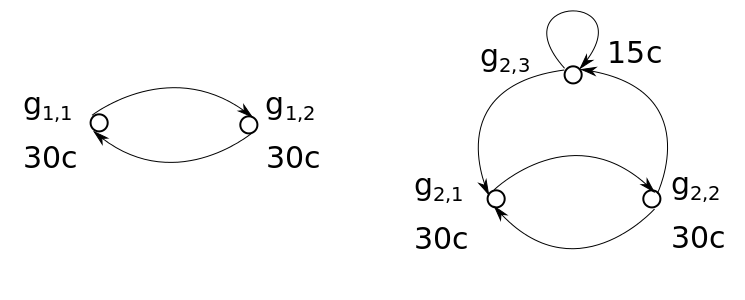
\includegraphics[scale=0.5]{SystemStates.png} 
\caption{Числовой пример тандема перекрестков. Левый граф соответствует первому перекрестку, правый~--- второму}
\label{SystemStates}
\end{figure}

Теперь продемонстрируем на конкретном числовом примере выделение циклов и состояний продления. Пусть изменение состояний перекрестков и время пребывания (в секундах для определнности) в каждом из состояний задается графами на рис. \ref{SystemStates}.



За начальное состояние объединенной системы примем $\Gamma_0=(g_{1,1},g_{2,1},0,0)$, то есть первый перекресток находится в состоянии $g_{1,1}$, второй~--- в состоянии $g_{2,1}$, и оба только начали свою работу в своем состоянии (этот факт моделируется равенствами $s=0$ и $t=0$). Следующая смена состояний случится у обоих перекрестков одновременно и приведет к следующему состоянию $(g_{1,2},g_{2,2}, 0, 0)$. Далее смена состояний произойдет также у первого и второго перекрестков, однако второй перекресток может перейти как в состояние $g_{2,1}$, так и в состояние продления $g_{2,3}$. Таким образом следущим состоянием тандема будет либо опять $(g_{1,1},g_{2,1},0,0)$, либо $(g_{1,1},g_{2,3},0,0)$. Продолжая рассуждения аналогичным образом, получим следущий список всех возможных состояний системы:

\begin{align*}
(g_{1,1},g_{2,1},0,0)&=\Gamma^{(1,1)} ,& \quad (g_{1,2},g_{2,2},0,0)&=\Gamma^{(1,2)} ,& \quad (g_{1,1},g_{2,3},0,0)&=\Gamma^{(0,1)}, \\
(g_{1,1},g_{2,3},15,2)&=\Gamma^{(0,2)} ,& \quad (g_{1,2},g_{2,3},0,0)&=\Gamma^{(0,3)} ,& \quad (g_{1,2},g_{2,3},15,2)&=\Gamma^{(0,4)}, \\
(g_{1,2},g_{2,1},15,2)&=\Gamma^{(4,1)} ,& \quad (g_{1,1},g_{2,1},15,1)&=\Gamma^{(4,2)} ,& \quad (g_{1,1},g_{2,2},15,2)&=\Gamma^{(4,3)}, \\
(g_{1,2},g_{2,2},15,1)&=\Gamma^{(4,4)} ,& \quad (g_{1,2},g_{2,3},15,2)&=\Gamma^{(0,5)} ,& \quad (g_{1,2},g_{2,1},0,0)&=\Gamma^{(3,1)}, \\
(g_{1,1},g_{2,2},0,0)&=\Gamma^{(3,2)} ,& \quad (g_{1,1},g_{2,1},15,2)&=\Gamma^{(2,1)} ,& \quad (g_{1,2},g_{2,1},15,1)&=\Gamma^{(2,2)}, \\
(g_{1,2},g_{2,2},15,2)&=\Gamma^{(2,3)} ,& \quad (g_{1,1},g_{2,2},15,1)&=\Gamma^{(2,4)}. & &
\end{align*}

В соответсвии с приведенными выше обозначениями, множества $C_1$, $C_2$, $C_3$, $C_4$, а также множество состояний продления строятся однозначным образом. Множествами входных состояний будут $C_1^{\mathrm{I}}=\{\Gamma^{(1,1)}\}$, $C_2^{\mathrm{I}}=\{\Gamma^{(2,1)}\}$, $C_3^{\mathrm{I}}=\{\Gamma^{(3,1)}\}$ и $C_4^{\mathrm{I}}\hm=\{\Gamma^{(4,1)}\}$. Множествами выходных состояний будут $C_1^{\mathrm{O}}=\{\Gamma^{(1,2)}\}$, $C_2^{\mathrm{O}}=\{\Gamma^{(2,4)}\}$, $C_3^{\mathrm{O}}=\{\Gamma^{(3,2)}\}$ и $C_4^{\mathrm{O}}=\{\Gamma^{(4,4)}\}$. Функции $h_1(\cdot)$, $h_2(\cdot)$ и $h_3(\cdot)$ задаются поточечно:
\begin{equation*}
h_1(\Gamma^{(1,2)})=1, \quad h_1(\Gamma^{(2,4)})=2, \quad h_1(\Gamma^{(3,2)})=3, \quad h_1(\Gamma^{(4,4)})=5,
\end{equation*}
\begin{equation*}
h_2(1)=2, \quad h_2(2)=3, \quad h_2(3)=4 \quad h_2(4)=1, \quad h_2(5)=1,
\end{equation*}
\begin{equation*}
h_3(1)=\Gamma^{(2,1)}, \quad h_3(2)=\Gamma^{(3,1)}, \quad h_3(3)=\Gamma^{(4,1)} \quad h_3(4)=\Gamma^{(1,1)}, \quad h_3(5)=\Gamma^{(1,1)}.
\end{equation*}
Этим завершается построение числового примера.


\section{Математическая модель}

Описанная в предыдущем разделе на содержательном уровне система массового обслуживания должна рассматриваться как кибернетическая управляющая система обслуживания (см.~\cite{Yablonski}). Схема управляющей системы приведена на Рис.~\ref{SystemScheme}. На схеме присутствуют следующие блоки: 1) внешняя среда с одним состоянием; 2) входные полюса первого типа~--- входные потоки $\Pi_1$, $\Pi_2$, $\Pi_3$, $\Pi_4$; 3) входные полюса второго типа~--- потоки насыщения $\Pi_1^{\mathrm{\text{нас}}}$, $\Pi_2^{\mathrm{\text{нас}}}$, $\Pi_3^{\mathrm{\text{нас}}}$, $\Pi_4^{\mathrm{\text{нас}}}$; 4) внешняя память~--- очереди $O_1$, $O_2$, $O_3$, $O_4$; 5) устройство по переработкe информации внешней памяти~--- устройства по поддержанию дисциплины очереди $\delta_1$, $\delta_2$, $\delta_3$, $\delta_4$; 6) внутренняя память~--- обслуживающее устройство (ОУ); 7) устройство по переработке информации во внутренней памяти~--- граф смены состояний; 8) выходные полюса $\Pi_1^{\mathrm{\text{вых}}}$, $\Pi_2^{\mathrm{\text{вых}}}$, $\Pi_3^{\mathrm{\text{вых}}}$, $\Pi_4^{\mathrm{\text{вых}}}$. Координатой блока является номер этого блока на схеме. 

Для задания информации блоков введем следующие величины и элементы, а также укажем множества их возможных значений. В качестве дискретной временной шкалы выберем последовательность $\tau_0=0$, $\tau_1$, $\tau_2$, $\ldots$ моментов смены состояния обслуживающего устройства. Обозначим $\Gamma_i$, $i\geqslant 1$, из множества $\Gamma$ состояние обслуживающего устройства в течение времени $\left(\tau_{i-1};\tau_i\right]$ и $\Gamma_0\in \Gamma$~--- в момент времени $\tau_0$, количество $\varkappa_{j,i} \in \mathbb{Z}_+ $, $i\geqslant 0$, требований в очереди $O_j$ в момент времени $\tau_i$, количество $\eta_{j,i} \in \mathbb{Z}_+$, $i\geqslant 0$, требований, поступивших в очередь $O_j$ по потоку $\Pi_j$ в течение времени $\left(\tau_{i};\tau_{i+1}\right]$, количество $\xi_{j,i} \in \mathbb{Z}_+$, $i\geqslant 0$, требований по потоку насыщения $\Pi^{\mathrm{\text{нас}}}_j$ в течение времени $\left(\tau_{i};\tau_{i+1}\right]$, количество $\overline{\xi}_{j,i}\in \mathbb{Z}_+$, $i\geqslant 0$, реально обслуженных требований по потоку $\Pi_j$ в течение времени $\left(\tau_{i};\tau_{i+1}\right]$; $j=\overline{1,4}$.

Закон изменения состояния обслуживающего устройства будем предполагать заданным соотношением 
\begin{equation}
\Gamma_{i+1}=h(\Gamma_i,\varkappa_{3,i}),
\label{gammaFunc}
\end{equation}
где отображение $h(\cdot,\cdot)$ определено в \eqref{hLaw}.
Для определения длительности $T_{i+1}$ состояния обслуживающего устройства в течение времени $\left(\tau_{i};\tau_{i+1}\right]$ удобно ввести функцию $h_T(\cdot,\cdot)$:
\begin{equation*}
T_{i+1}=h_T(\Gamma_i,\varkappa_{3,i})= T^{(k,r)},\quad  \text{ где $k$ и $r$ таковы, что } \Gamma^{(k,r)}=\Gamma_{i+1}=h(\Gamma_i,\varkappa_{3,i}).
%\label{timeLaw}
\end{equation*}
Функциональная зависимость
\begin{equation}
\overline{\xi}_{j,i}=\min\{\varkappa_{j,i}+\eta_{j,i},\xi_{j,i}\}, \quad j\in \{1,2,3\},
\label{saturationEq}
\end{equation}
между величиной $\overline{\xi}_{j,i}$ и величинами $\varkappa_{j,i}$, $\eta_{j,i}$, $\xi_{j,i}$ реализует стратегию механизма обслуживания требований. Далее, поскольку 
\begin{equation*}
\varkappa_{j,i+1}=\varkappa_{j,i}+\eta_{j,i}-\overline{\xi}_{j,i}, \quad  j\in \{1,2,3\},
\end{equation*}
то из выражения \eqref{saturationEq} следует соотношение
\begin{equation}
\varkappa_{j,i+1}=\max\{{0,\varkappa_{j,i}+\eta_{j,i}-\xi_{j,i}}\}, \quad j\in \{1,2,3\}.
\label{queuesFunc}
\end{equation}
Из формулировки поставленной задачи (см. также структурную схему на Рис.~\ref{SystemScheme}) следуют соотношения для потока $\Pi_4$:
\begin{equation}
\eta_{4,i} = \min\{\xi_{1,i}, \varkappa_{1,i}+\eta_{1,i}\}, \quad \varkappa_{4,i+1}=\varkappa_{4,i}+\eta_{4,i}-\eta_{2,i}, \quad \xi_{4,i} = \varkappa_{4,i}.
\label{FourthFunc}
\end{equation}

Нелокальное описание входных потоков и потоков насыщения заключается  в указании некоторых свойств условных распределений выделенных дискретных компонент $\eta_i$ и $\xi_i$ маркированных точечных процессов \linebreak $\{(\tau_i, \nu_i, \eta_i); i\geqslant 0\}$ и $\{(\tau_i, \nu_i, \xi_i); i\geqslant 0\}$ при фиксированных значениях метки $\nu_i \hm= (\Gamma_i;\varkappa_i)$, где $\eta_i\hm=(\eta_{1,i}, \eta_{2,i}, \eta_{3,i}, \eta_{4,i})$, $\xi_i \hm= (\xi_{1,i}, \xi_{2,i}, \xi_{3,i}, \xi_{4,i})$ и $\varkappa_i \hm= (\varkappa_{1,i},\varkappa_{2,i},\varkappa_{3,i},\varkappa_{4,i})$. 
Введем функции $\varphi_1(\cdot,\cdot)$ и $\varphi_3(\cdot,\cdot)$ из разложений 
\begin{equation*}
\sum_{\nu=0}^{\infty} z^\nu\varphi_j(\nu,t) = \exp\{\lambda_j t (f_j(z)-1)\},
\end{equation*}
где $f_j(z)$ определены выражением \eqref{GeneratingFunc}, $j \in \{1,3\}$. Функция $\varphi_j(\nu,t)$ по своему смыслу есть вероятность поступления $\nu=0$, $1$, $\ldots$ требований по потоку $\Pi_j$ за время $t \geqslant 0$. Положим $\varphi_j(\nu,t)$ равной нулю при $\nu < 0$. Функцию $\psi(\cdot,\cdot,\cdot)$ зададим формулой
\begin{equation*}
\psi(k;y,u)=C_y^k u^k (1-u)^{y-k}.	
\end{equation*}
По своему смыслу $\psi(k;y,u)$ есть вероятность поступления $k$ требований по потоку $\Pi_2$ при условии, что очередь $O_4$ содержит $y$ требований и обслуживающее устройство находится в состоянии $\Gamma^{(k,r)}$, так что $u=p_{k,r}$. При нарушении условия $ 0\leqslant k \leqslant y$ положим $\psi(k;y,u)$ равной нулю.

Пусть $a=(a_1, a_2, a_3, a_4) \in \mathbb{Z}_+^4$ и $x=(x_1, x_2, x_3, x_4) \in \mathbb{Z}_+^4$. Тогда из постановки задачи на содержательном уровне следует, что при фиксированном значении метки $\nu_i=(\Gamma^{(k,r)}; x)$ вероятность $\varphi(a,k,r,x)$ одновременного выполнения равенств $\eta_{1,i}=a_1$, $\eta_{2,i}=a_2$, $\eta_{3,i}=a_3$, $\eta_{4,i}=a_4$ есть 
\begin{equation}
\varphi_1(a_1,h_T(\Gamma^{(k,r)},x_3)) \psi(a_2,x_4, p_{\tilde{k},\tilde{r}})  \varphi_3(a_3,h_T(\Gamma^{(k,r)},x_3))
 \delta_{a_4,\min{\{\ell(\tilde{k},\tilde{r},1), x_1+a_1}\}},
\label{conditionProbOne}
\end{equation}
где $\tilde{k}$ и $\tilde{r}$ таковы, что $\Gamma^{(\tilde{k},\tilde{r})}=h(\Gamma^{(k,r)},x_3)$ и $\delta_{i,j}$ есть символ Кронекера:
%\begin{equation*}
$$
\delta_{i,j}=
\begin{cases} 
1,& \quad \text{ если $i=j$,}\\
0,& \quad \text{ если $i\neq j$.}
\end{cases}
$$%\end{equation*}
Пусть $b=(b_1, b_2, b_3, b_4) \in \mathbb{Z}_+^4$. Из содержательной постановки задачи также следует, что вероятность $\zeta(b, k, r, x)$ одновременного выполнения равенств $\xi_{1,i}=b_1$, $\xi_{2,i}=b_2$, $\xi_{3,i}=b_3$, $\xi_{4,i}=b_4$ при фиксированном значении $(\Gamma^{(k,r)}; x)$ метки $\nu_i$ есть
\begin{equation}
\delta_{b_1,\ell(\tilde{k},\tilde{r},1)} \times \delta_{b_2,\ell(\tilde{k},\tilde{r},2)} \times 
\delta_{b_3,\ell(\tilde{k},\tilde{r},3)} \times \delta_{b_4,x_4}.
\label{conditionProbTwo}
\end{equation}
Из формулы \eqref{conditionProbTwo} следует для $j\in \{1, 2, 3\}$, что вероятность события $\xi_{j,i}=0$ равна $1$ в случае $h(\Gamma^{(k,r)},x_3)\notin {}^j\Gamma$ и что вероятность события $\xi_{j,i}=\ell(\tilde{k},\tilde{r},j)$ равна $1$, если $\Gamma^{(\tilde{k},\tilde{r})}=h(\Gamma^{(k,r)},x_3)\in {}^j\Gamma$.


Содержательный смысл следующей теоремы состоит в том, что сформулированные выше функциональные связи и вероятностные свойства введенных объектов непротиворечивы и могут быть реализованы на некотором вероятностном пространстве.
%Построим теперь 	вероятностное пространство $(\Omega, {\cal F}, \Pr(\cdot))$, чтобы можно было рассматривать введеные величины как случайные величины на этом пространстве. А именно, докажем следующую теорему.

\begin{theorem}
Пусть $\gamma_0=\Gamma^{(k_0,r_0)}\in \Gamma$ и $x^0=(x_{1,0},x_{2,0}, x_{3,0},x_{4,0})\in \mathbb{Z}_+^4$ фиксированы.
Тогда существует вероятностное пространство $(\Omega, {\cal F}, \Pr(\cdot))$ и заданные на нем случайные величины $\eta_{j,i}=\eta_{j,i}(\omega)$, $\xi_{j,i}=\xi_{j,i}(\omega)$, 	 $\varkappa_{j,i}=\varkappa_{j,i}(\omega)$ и случайные элементы $\Gamma_i=\Gamma_i(\omega)$, $i\geqslant 0$, $j= \overline{1,4}$, такие, что 1) имеют место равенства $\Gamma_0(\omega) = \gamma_0$ и $\varkappa_0(\omega)=x^0$; 2) выполняются соотношения \eqref{gammaFunc}, \eqref{queuesFunc}, \eqref{FourthFunc}; 3) для любых  $a\in \mathbb{Z}_+^4$, $b\in \mathbb{Z}_+^4$ и любых $x^t=(x_{1,t},x_{2,t},x_{3,t},x_{4,t}) \in \mathbb{Z}_+^4$, $\Gamma^{(k_t,r_t)} \in \Gamma$, $t = 1, 2, \ldots$, таких, что $\Pr\Bigl(\bigcap\limits_{t=0}^{i}\{\omega\colon \Gamma_t=\Gamma^{(k_t,r_t)}, \varkappa_t=x^t\}\Bigr)>0$, условное распределение векторов $\eta_i$ и $\xi_i$, $i \geqslant 0$,  имеет вид
\begin{equation}
\Pr \biggl(\{ \omega \colon \eta_i = a, \xi_i=b\} \bigg
|\,\bigcap_{t=0}^{i}\{\omega\colon \Gamma_t=\Gamma^{(k_t,r_t)}, \varkappa_t=x^t\}\biggr)=
\varphi(a,k_i,r_i,x^i)\times \zeta(b,k_i,r_i,x^i),
\label{ProbablititiesToProve}
\end{equation}
где функции $\varphi(\cdot, \cdot, \cdot, \cdot)$ и $\zeta(\cdot, \cdot, \cdot, \cdot)$ определяются формулами \eqref{conditionProbOne} и \eqref{conditionProbTwo}.

\label{myTheorem}
\end{theorem}
\begin{proof}

Для построения вероятностного пространства $(\Omega, {\cal F}, \Pr(\cdot))$ воспользуемся теоремой И. Тулчи (см. \cite{Shiryaev}, c. 348). 

Введем последовательность измеримых пространств $(\Omega_0, {\cal F}_0)$, $(\Omega_1, {\cal F}_1)$,$\ldots$, где $\Omega_i\hm=\mathbb{Z}_+^3$, $\omega_i=(\omega_{1,i},\omega_{2,i},\omega_{3,i}) \hm\in \Omega_i$, а $\sigma$-алгебра ${\cal F}_i=2^{\Omega_i}$  есть множество всех подмножеств множества $\Omega_i$. 
Пусть $\Gamma^{(\tilde{k},\tilde{r})}=h(\Gamma^{(k_0,r_0)},x_{3,0})$.
Зададим на измеримом пространстве $(\Omega_0, {\cal F}_0)$ вероятностную меру $P_0(\cdot)$ ее значениями на одноточечных множествах:
\begin{equation}
P_0(\{(a_1,a_2,a_3)\})=\varphi_1(a_1,h_T(\Gamma^{(k_0,r_0)})) \times \psi(a_2,x_{2,0}, p_{\tilde{k},\tilde{r}}) \times \varphi_3(a_3,h_T(\Gamma^{(k_0,r_0)})).
\label{probabilitiesOne}
\end{equation}

Для $j\in \{1,2,3\}$ определим величины
\begin{equation}
\tilde{\Gamma}_0(\omega_0)=\gamma_0, \quad \tilde{\varkappa}_{j,0}(\omega_0)=x_{j,0}, \quad \tilde{\xi}_{j,0}(\omega_0)=l(\tilde{k},\tilde{r},j), \quad \tilde{\eta}_{j,0}(\omega_0)=\omega_{j,0},
\label{startRekOne}
\end{equation}
и
\begin{equation}
 \tilde{\varkappa}_{4,0}(\omega_0)=x_{4,0}, \quad \tilde{\xi}_{4,0}(\omega_0)=x_{4,0}, \quad \tilde{\eta}_{4,0}(\omega_0)=\min\{\tilde{\xi}_{1,0}(\omega_0), \tilde{\varkappa}_{1,0}(\omega_0)+\tilde{\eta}_{1,0}(\omega_0)\}.
\label{startRekTwo}
\end{equation}

Теперь предположим, что заданы вероятностные меры $P_i(\omega_0\hm{}, \omega_1,\hm{} \ldots \hm{}, \omega_{i-1};\cdot)$ на измеримом пространстве $(\Omega_i, {\cal F}_i)$, $i=\overline{0,n}$,
и 
% определеныслучайные величины $\tilde{\Gamma}_i$, $\tilde{\varkappa}_{j,i}$, $\tilde{\xi}_{j,i}$, $\tilde{\eta}_{j,i}$, ч, и 
фиксирован набор $(\omega_0, \omega_1, \hm\ldots, \omega_{n})$. Положим для $j\in \{1, 2, 3\}$  и $i=\overline{0,n}$
\begin{equation}
\tilde{\Gamma}_{i+1}=\Gamma^{(k^*,r^*)}=h(\tilde{\Gamma}_{i},\tilde{\varkappa}_{3,i}), \quad \tilde{\varkappa}_{j,i+1}=\max\{ 0,\tilde{\varkappa}_{j,i}+\tilde{\eta}_{j,i} -\tilde{\xi}_{j,i}\},
\label{NextRekOne}
\end{equation}
\begin{equation}
\tilde{\varkappa}_{4,i+1}=\tilde{\varkappa}_{4,i}+\tilde{\eta}_{4,i}-\tilde{\eta}_{2,i}, \quad \tilde{\xi}_{j,i+1}=l(k^*,r^*,j),\quad \tilde{\eta}_{j,i+1}=\omega_{j,i+1}
\label{NextRekTwo}
\end{equation}
\begin{equation}
\tilde{\eta}_{4,i+1}=\min\{\tilde{\xi}_{1,i+1}, \tilde{\varkappa}_{1,i+1}+\tilde{\eta}_{1,i+1}\}, \quad \tilde{\xi}_{4,i+1}=\tilde{\varkappa}_{4,i+1}.
\label{NextRekThree}
\end{equation}
Заметим, что значения $\tilde{\Gamma}_{j,i}$, $\tilde\xi_{j,i}$, $\tilde\eta_{j,i}$, $\tilde\varkappa_{j,i}$, найденные по формулам \eqref{NextRekOne}--\eqref{NextRekThree} по наборам $(\omega_0, \omega_1,\ldots, \omega_n)$ и $(\omega_0, \omega_1,\ldots, \omega_i)$, $n\geqslant i$, совпадают.
Определим на измеримом пространстве $(\Omega_{n+1}, {\cal F}_{n+1})$ вероятностную меру  $P_{n+1}(\omega_0, \omega_1, \hm\ldots, \omega_n;\cdot)$
ее значениями на одноточечных множествах $\{(a_1,a_2,a_3)\}$, $(a_1,a_2,a_3)\hm\in {\mathbb Z}_+^3$:
\begin{multline}
P_{n+1}(\omega_0,\omega_1,\ldots,\omega_n;\{(a_1,a_2,a_3)\}) = \\
= \varphi_1(a_1,h_T(\tilde{\Gamma}_n,\tilde{\varkappa}_{3,n})) \times \psi(a_2,\tilde{\varkappa}_{4,n}, p_{k^*,r^*}) \times \varphi_3(a_3,h_T(\tilde{\Gamma}_n,\tilde{\varkappa}_{3,n})).
\label{probabilitiesTwo}
\end{multline}

%причем для любого множества $B\in {\cal F}_i$ функции $P(\omega_0,\omega_1,\hm\ldots,  \omega_{i-1};B)$ должны быть измеримыми функциями от $(\omega_0, \omega_1, \ldots, \omega_{i-1})$. 



Тогда (в соответствии с теоремой Ионеску Тулчи) для декартова произведения $\Omega=\prod\limits_{i=0}^{\infty}\Omega_i$ пространств элементарных исходов и произведения $\sigma$-алгебр ${\cal F}=\bigotimes\limits_{i=0}^{\infty} {\cal F}_i$ на $(\Omega,{\cal F})$ будет существовать единственная вероятностная мера $\Pr(\cdot)$ такая, что для любого $i \geqslant 0$ верно равенство
\begin{equation}
\Pr(\{\omega \colon \omega_0 \in A_0, \omega_1 \in A_1, \ldots, \omega_i\in A_i\})= P_i(A_0 \times A_1 \times \ldots \times A_i),
\label{ProbabilitiesGeneral}
\end{equation}
где 
\begin{equation}
 P_i(A_0 \times A_1 \times \ldots \times A_i) = \int_{A_0} P_0(d \omega_0) \int_{A_1} P_1(\omega_0;d \omega_1) \ldots \int_{A_i} P_i(\omega_0, \omega_1, \ldots, \omega_{i-1}; d \omega_i),
\label{ProbabilitiesGeneralOne}
\end{equation}
для любого $A_i$ из ${\cal F}_i$. Итак, вероятностное пространство $(\Omega,{\cal F},\Pr(\cdot))$ построено. 

Теперь введем на пространстве $(\Omega,{\cal F},\Pr(\cdot))$ следующие случайные величины и элементы, $i \geqslant 0$, $j =\overline{1,4}$:
\begin{equation*}
    \Gamma_i(\omega) = \tilde{\Gamma}_i, \quad \varkappa_{j,i}(\omega) = \tilde{\varkappa}_{j,i},\quad
    \xi_{j,i}(\omega) = \tilde{\xi}_{j,i}, \quad \eta_{j,i}(\omega) = \tilde{\eta}_{j,i}.
\end{equation*}
и докажем, что они  удовлетворяют условиям теоремы. Для сокращения записи зависимость от $\omega$ в обозначении случайных элементов и случайных величин далее будем опускать. Из формулы \eqref{NextRekOne} следует, что случайные элементы $\Gamma_i$ удовлетворяют соотношению \eqref{gammaFunc}, а случайные величины $\varkappa_{j,i}$ для $j\in \{1, 2, 3\}$ удовлетворяют соотношению \eqref{queuesFunc}. Из формулы \eqref{NextRekTwo} заключаем, что $\varkappa_{4,i}$ удовлетворяет соотношению $\eqref{FourthFunc}$. Далее, из условий \eqref{startRekTwo} и \eqref{NextRekThree} следует справедливость соотношений \eqref{FourthFunc} для величин $\eta_{4,i}$ и $\xi_{4,i}$. 

Перейдем к доказательству равенства \eqref{ProbablititiesToProve}. Для сокращения записи введем множества $B_i = \bigcap_{t=0}^{i}\{\omega\colon \Gamma_t=\Gamma^{(k_t,r_t)}, \varkappa_t=x^t\}$, $i\geqslant 0$. Найдем явное выражение для условной вероятности $\Pr (\{ \omega \colon \eta_i = a, \xi_i=b\} | B_i)$. Пусть $\Gamma^{(\tilde{k}_i,\tilde{r}_i)}=h(\Gamma^{(k_i,r_i)},x^i)$. Запишем по определению условной вероятности, предполагая, что $\Pr(B_i)>0$:
\begin{multline}
\Pr \bigl(\left\{ \omega \colon \eta_i = a, \xi_i=b\right\}  |B_i\bigr) 
=\Pr\bigl(\{ \omega \colon \eta_i = a, \xi_i=b \} \cap B_i\bigr) 
\times
\bigl(\Pr\bigl( B_i\bigr)\bigr)^{-1}.
\label{Construction:1}
\end{multline}
Далее из соотношений \eqref{ProbabilitiesGeneral}, \eqref{ProbabilitiesGeneralOne} и того факта, что значения $\Gamma_i$ и $\varkappa_{i}$ зависят только от $\omega_0$, $\omega_1$ , $\ldots$, $\omega_{i-1}$, но не от $\omega_i$, (этот факт следует из формул \eqref{startRekOne}~--~\eqref{NextRekTwo}), получим выражение для второго сомножителя последнего выражения
\begin{multline}
\Pr\bigl( B_i\bigr)=\\
=\sum_{\substack{\omega_0, \omega_1,\ldots, \omega_{i-1} \colon \\ \Gamma_t=\Gamma^{(k_t,r_t)},\, \varkappa_t=x^t,\\ t=\overline{0,i-1}}} P_0(\omega_0)\times P_1(\omega_0;\{\omega_1\})\times\ldots\times P_{i-1}(\omega_0,\omega_1,\ldots, \omega_{i-2};\{\omega_{i-1}\}).
\label{Construction:2}
\end{multline}
%Здесь мы положили $A_t(\omega_0,\omega_1,\ldots,\omega_{t-1})=\{\omega_t \colon \Gamma_t=\Gamma^{(k_t,r_t)}, \varkappa_t=x^t\}$, $t=\overline{0,i}$.

Преобразуем множество $\{\omega\colon \eta_i = a, \xi_i=b \} \cap \{\omega\colon\Gamma_i=\Gamma^{(k_i,r_i)}, \varkappa_i=x^i\}$, учитывая соотношения \eqref{startRekOne}~--~\eqref{NextRekThree}:
\begin{multline*}
\left\{\omega\colon \eta_i = a, \xi_i=b \right\} \cap \left\{\omega\colon\Gamma_i=\Gamma^{(k_i,r_i)}, \varkappa_i=x^i\right\} = \left\{\omega\colon\Gamma_i=\Gamma^{(k_i,r_i)}, \varkappa_i=x^i\right\} \cap\\   \displaybreak[0]
\cap \left\{\omega\colon \eta_{j,i} = a_j, j=\overline{1,3}\right\} \cap \left\{\omega\colon \xi_{j,i} = b_j, j=\overline{1,3}\right\} \cap \left\{ \omega\colon\xi_{4,i} = b_4 \right\} \cap  \left\{\omega\colon \eta_{4,i} = a_4 \right\} = \\  \displaybreak[0]
= \left\{\omega\colon\Gamma_i=\Gamma^{(k_i,r_i)}, \varkappa_i=x^i\right\} \cap \left\{\omega\colon \omega_{j,i} = a_j, j= \overline{1,3}\right\} \cap \\ \cap  \left\{\omega\colon b_j=\ell(\tilde{k}_i,\tilde{r}_i,j), j=\overline{1,3}\right\} 
\cap \left\{ \omega\colon b_4 = x_{4,i} \right\} \cap \\  \displaybreak[0] \cap \left\{\omega\colon a_4=\min\left\{\ell(\tilde{k}_i,\tilde{r}_i,1), x_{1,i}+a_1\right\} \right\}. 
\end{multline*}
Тогда для второго множителя из правой части выражения \eqref{Construction:1} имеем:
\begin{multline}
\Pr\bigl(\{ \omega \colon \eta_i = a, \xi_i=b \} \cap B_i\bigr)=\\ 
=
\Pr\bigl(\left\{\omega\colon \eta_i = a, \xi_i=b \right\} \cap  \left\{\omega\colon\Gamma_i=\Gamma^{(k_i,r_i)}, \varkappa_i=x^i\right\}  \cap B_{i-1}\bigr)=\displaybreak[0]\\
= \delta_{b_4,x_{4,i}} \times \delta_{a_4,\min\left\{\ell(\tilde{k}_i,\tilde{r}_i,1), x_{1,i}+a_1\right\}} \times \prod_{j=1}^3\delta_{b_j,\ell(\tilde{k}_i,\tilde{r}_i,j)}   \times \displaybreak[0]\\
\times \Pr\bigl( \left\{ \omega\colon \omega_{j,i} = a_j, j=\overline{1,3}\right\} \cap \left\{\omega\colon\Gamma_i=\Gamma^{(k_i,r_i)}, \varkappa_i=x^i\right\} \cap B_{i-1}\bigr).
\label{Construction:3}
\end{multline}
И по аналогии со вторым множителем в выражении \eqref{Construction:2} преобразуем последний сомножитель правой части равенства \eqref{Construction:3}:
\begin{multline*}
\Pr\bigl( \left\{ \omega \colon \omega_{j,i} = a_j,j=\overline{1,3}; \Gamma_i=\Gamma^{(k_i,r_i)}, \varkappa_i=x^i\right\} \cap B_{i-1}\bigr) 
= \\ =\sum_{\substack{\omega_0, \omega_1,\ldots, \omega_{i-1} \colon \\ \Gamma_t=\Gamma^{(k_t,r_t)},\, \varkappa_t=x^t, \\ t=\overline{0,i-1}}} P_0(\omega_0)\times P_1(\omega_0;\{\omega_1\})\times\ldots \times P_{i-1}(\omega_0,\omega_1,\ldots, \omega_{i-2};\{\omega_{i-1}\})
\times \\[-2ex] \times P_i(\omega_0,\omega_1,\ldots, \omega_{i-1};\{(a_1, a_2, a_3)\})
\end{multline*}
и, учитывая выражение \eqref{probabilitiesTwo}, получим
\begin{multline}
\Pr\bigl( \left\{ \omega \colon \omega_{j,i} = a_j, j=\overline{1,3}; \Gamma_i=\Gamma^{(k_i,r_i)}, \varkappa_i=x^i\right\} \cap B_{i-1}\bigr) 
=\\=\varphi_1(a_1,h_T(\Gamma_i,x_{3,i})) \times \psi(a_2,x_{4,i}, p_{\tilde{k}_i,\tilde{r}_i}) \times  \varphi_3(a_3,h_T(\Gamma_i,x_{3,i}))
\times \\ \times \sum_{\substack{\omega_0, \omega_1,\ldots, \omega_{i-1} \colon \\ \Gamma_t=\Gamma^{(k_t,r_t)},\, \varkappa_t=x^t,\\ t=\overline{0,i-1}}} P_0(\omega_0)\times P_1(\omega_0;\{\omega_1\})\times \ldots \times P_{i-1}(\omega_0,\omega_1,\ldots, \omega_{i-2};\{\omega_{i-1}\}).
\label{Construction:4}
\end{multline}

Подставляя выражение \eqref{Construction:4} в правую часть равенств \eqref{Construction:3}, а затем выражения  \eqref{Construction:3} и \eqref{Construction:2} в равенство \eqref{Construction:1}, получим:
\begin{multline*}
\Pr \bigl(\left\{ \omega \colon \eta_i = a, \xi_i=b\right\}  \bigl| B_i \bigr.\bigr)  = \\
= \delta_{b_4,x_{4,i}} \times \delta_{a_4,\min\left\{\ell(\tilde{k}_i,\tilde{r}_i,1), x_{1,i}+a_1\right\}} \times \prod_{j=1}^3\delta_{b_j,\ell(\tilde{k}_i,\tilde{r}_i,j)} \times
\varphi_1(a_1,h_T(\Gamma_i,x_{3,i})) \times \\ \times \psi(a_2,x_{4,i}, p_{\tilde{k}_i,\tilde{r}_i}) 
\times  \varphi_3(a_3,h_T(\Gamma_i,x_{3,i})) \times\displaybreak[0] \\ 
\times \sum_{\substack{\omega_0, \omega_1,\ldots \omega_{i-1} \colon \\ \Gamma_t=\Gamma^{(k_t,r_t)}, \varkappa_t=x^t, \forall 0\leqslant t \leqslant i-1}} P_0(\omega_0)\times P_1(\omega_0;\{\omega_1\})\times\ldots\times P_{i-1}(\omega_0,\omega_1,\ldots, \omega_{i-2};\{\omega_{i-1}\}) \times \\
\times \raisebox{-1ex}{$\mathsurround=0pt \Biggl($} \sum_{\substack{\omega_0, \omega_1,\ldots \omega_{i-1} \colon \\ \Gamma_t=\Gamma^{(k_t,r_t)}, \varkappa_t=x^t, \forall 0\leqslant t \leqslant i-1}} P_0(\omega_0)\times P_1(\omega_0;\{\omega_1\})\times\ldots\times \\ \times P_{i-1}(\omega_0,\omega_1,\ldots, \omega_{i-2};\{\omega_{i-1}\})\raisebox{-1ex}{$\mathsurround=0pt \Biggr)$}^{-1}
\end{multline*}
и после сокращения одинаковых сумм получаем требуемое равенство \eqref{ProbablititiesToProve}.
\end{proof}







\section{Очереди первичных требований}

Рассмотрим случайную последовательность  $$\{(\Gamma_i, \varkappa_{1,i},\varkappa_{3,i}); i \geqslant 0\},$$ включающую в себя состояния $\varkappa_{1,i}$ и $\varkappa_{3,i}$ очередей $O_1$ и $O_3$ первичных требований в момент $\tau_i$. Приведем ниже несколько результатов, касающихся этой последовательности.

\begin{statement}
Пусть $\Gamma_0=\Gamma^{(k,r)}\in \Gamma$ и $(\varkappa_{1,0}, \varkappa_{3,0})=(x_{1,0}, x_{3,0})\in \mathbb{Z}_+^2$ фиксированы. Тогда последовательность $\{(\Gamma_i, \varkappa_{1,i},\varkappa_{3,i}); i \geqslant 0\}$ является однородной счетной цепью Маркова.
\end{statement}


Обозначим для $\gamma \in \Gamma$ и $(x_1,x_3) \in {\mathbb Z}_+^2$
\begin{equation}
Q_{1,i}(\gamma,x_1,x_3) = \Pr(\Gamma_{i}=\gamma, \varkappa_{1,i}=x_1, \varkappa_{3,i}=x_3),
\end{equation}
а также введем множество
\begin{equation*}
{\mathbb H}_{-1}(\Gamma^{(k,r)}, x_3) = \{\gamma \in \Gamma \colon h(\gamma, x_3) = \Gamma^{(k,r)}\}.
\end{equation*}
Положим $r \ominus_k 1 = r-1$ для $r=\overline{2,n_k}$ и $r \ominus_k 1 = n_k$ при $r=1$, $k = \overline{0,d}$. Из определения \eqref{hLaw} находим явный вид множества для различных $\Gamma^{(k,r)}$ и $x_3$:
\begin{equation}
{\mathbb H}_{-1}(\Gamma^{(k,r)}, x_3) = 
\begin{cases}
\{\Gamma^{(k_1,r_1)}, \Gamma^{(0,r\ominus_0 1)}\},& \quad \text{ если } (k=0\text{ \& } x_3 \leqslant L);\\
\{\Gamma^{(k,r\ominus_k 1)}, \Gamma^{(0,r_2)}\},& \quad \text{ если } (\Gamma^{(k,r)}\in C_k^{\mathrm{I}} \text{ \& } x_3>L);\\ 
\{\Gamma^{(k,r\ominus_k 1)}\},& \quad \text{ если } (\Gamma^{(k,r)}\in C_k^{\mathrm{O}}) \text{ или } (\Gamma^{(k,r)}\in C_k^{\mathrm{N}});\\
\varnothing,& \quad \text{ если $(k = 0 \:\&\: x_3>L)$}\\ 
 & \text{ \phantom{1}\qquad или $(\Gamma^{(k,r)}\in C_k^{\mathrm{I}} \:\&\: x_3\leqslant L)$},
\end{cases}
\end{equation}
где $k_1,r_1$ таковы, что $h_1(\Gamma^{(k_1,r_1)})=r$, и $r_2$ таково, что $h_3(r_2)=\Gamma^{(k,r)}$.

Важным шагом при исследовании стационарного режима цепи $\{(\Gamma_i, \varkappa_{1,i},\varkappa_{3,i}); i \geqslant 0\}$ является нахождение множества ее существенных состояний. Введем множества 
\begin{equation*}
  S^1_{0,r} = 
  \biggl\{
  (\Gamma^{(0,r)},x_1, x_3) \colon \; (x_1, x_3)\in Z^2_+,\; x_3 > L - \max\limits_{k=1, 2,
    \ldots, d}
  \biggl\{ \sum_{t=1}^{n_k} \ell({k,t,3}) \biggl\}\biggl\}, 
\end{equation*}
для $1 \leqslant r \leqslant n_0$ и множества
\begin{equation*}
  S^1_{k,r} =
  \biggl\{
  (\Gamma^{(k,r)},x_1, x_3) \colon \; (x_1, x_3)\in Z^2_+,\; x_3 > L - \sum_{t=1}^{r} \ell({k,t,3})
  \biggr\},
\end{equation*}
для $1 \leqslant k \leqslant d$,  $1 \leqslant r \leqslant n_k$.
Тогда верно следующее
\begin{statement}
Множество существенных состояний марковской цепи $\{(\Gamma_i, \varkappa_{1,i},\varkappa_{3,i}); i \geqslant 0\}$ имеет вид $\raisebox{-.5ex}{$\biggl($}\bigcup\limits_{1 \leqslant r \leqslant n_0}S^1_{0,r}\raisebox{-.5ex}{$\biggr)$}\cup \raisebox{-.5ex}{$\biggl($}\bigcup\limits_{\substack{1 \leqslant k \leqslant d\\ 1 \leqslant r \leqslant n_k}} S^1_{k,r}\raisebox{-.5ex}{$\biggr)$}$.
\end{statement}

Пусть $k$ и $r$ таковы, что $\Gamma^{(k,r)}\in \Gamma$. Введем частичные производящие функции
\begin{equation*}
\mathfrak{M}^{(1,i)}(k,r,v_1,v_3) = \sum_{w_1=0}^{\infty}\sum_{w_3=0}^{\infty} Q_{1,i}(\Gamma^{(k,r)},w_1,w_3) v_1^{w_1} v_3^{w_3},
\end{equation*}
и вспомогательные функции
\begin{align*}
q^{(1)}(k,r, v_1) &= v_1^{-\ell(k,r,1)}\sum_{w=0}^{\infty} \varphi_1(w,T^{(k,r)})v_1^w;\\
q^{(3)}(k,r, v_3) &= v_3^{-\ell(k,r,3)}\sum_{w=0}^{\infty} \varphi_3(w,T^{(k,r)})v_3^w.
\end{align*}
В введенных обозначениях верна следующая
\begin{lemma}
Пусть  $\tilde{\gamma}=\Gamma^{(\tilde{k},\tilde{r})}\in \Gamma$. Тогда верно следующее рекуррентное соотношение:
\begin{multline*}
\mathfrak{M}^{(1,i+1)}(\tilde{k},\tilde{r},v_1,v_3) 
= \sum_{w_1=0}^{\infty}\sum_{w_3=0}^{\infty} \sum_{\Gamma^{(k,r)} \in {\mathbb H}_{-1}(\tilde{\gamma},w_3)} Q_{1,i}(\Gamma^{(k,r)},w_1,w_3) \times \\ \times \biggl[ v_1^{w_1} q^{(1)}(\tilde{k},\tilde{r},v_1) + I(\tilde{\gamma}\in \Gamma^{\mathrm{\Rmnum{1}}}) \sum_{a=0}^{\ell(\tilde{k},\tilde{r},1)-w_1} \varphi_1(a,T^{(\tilde{k},\tilde{r})})(1-v_1^{w_1+a-\ell(\tilde{k},\tilde{r},1)})\biggr] \times \\ 
\times \biggl[ v_3^{w_3} q^{(3)}(\tilde{k},\tilde{r},v_3) + I(\tilde{\gamma}\in \Gamma^{\mathrm{\Rmnum{3}}}) \sum_{a=0}^{\ell(\tilde{k},\tilde{r},3)-w_3} \varphi_3(a,T^{(\tilde{k},\tilde{r})})(1-v_3^{w_3+a-\ell(\tilde{k},\tilde{r},3)})\biggr].
\end{multline*}
\label{second:approach:lemma:first:step}
\end{lemma}
\begin{proof}
Пусть $\Gamma^{(k,r)} \in \Gamma$. Учитывая соотношения $\eqref{queuesFunc}$ и вид условных распределений \eqref{ProbablititiesToProve} для $\eta_i$ и $\xi_i$, $i\geqslant 0$, запишем по формуле повторного математического ожидания:
\begin{multline}
\mathfrak{M}^{(1,i+1)}(\tilde{k},\tilde{r},v_1,v_3) =\\ = E[v_1^{\varkappa_{1,i+1}}v_3^{\varkappa_{1,i+1}}I(\Gamma_{i+1}=\tilde{\gamma})] = 
\sum_{w_1=0}^{\infty}\sum_{w_3=0}^{\infty} \sum_{\Gamma^{(k,r)} \in \Gamma} Q_{1,i}(\Gamma^{(k,r)},w_1,w_3) \times \\ \times
E[v_1^{\varkappa_{1,i+1}}v_3^{\varkappa_{1,i+1}}I(\Gamma_{i+1}=\tilde{\gamma}) | \varkappa_{1,i}=w_1,\varkappa_{3,i}=w_3, \Gamma_i=\Gamma^{(k,r)}] = \\ =
\sum_{w_1=0}^{\infty}\sum_{w_3=0}^{\infty} \sum_{\Gamma^{(k,r)} \in {\mathbb H}_{-1}(\tilde{\gamma},x_3)} Q_{1,i}(\Gamma^{(k,r)},w_1,w_3) 
\times \\ \times E[v_1^{\max{\{0, w_1 + \eta_{1,i} - \ell(\tilde{k},\tilde{r},1)\}}} v_3^{\max{\{0, w_3 + \eta_{3,i} - \ell(\tilde{k},\tilde{r},3)\}}} | \varkappa_{1,i}=w_1,\varkappa_{3,i}=w_3, \Gamma_i=\Gamma^{(k,r)}] = \\ =
\sum_{w_1=0}^{\infty}\sum_{w_3=0}^{\infty} \sum_{\Gamma^{(k,r)} \in {\mathbb H}_{-1}(\tilde{\gamma},x_3)} Q_{1,i}(\Gamma^{(k,r)},w_1,w_3) 
\times \\ \times E[v_1^{\max{\{0, w_1 + \eta_{1,i} - \ell(\tilde{k},\tilde{r},1)\}}} | \varkappa_{1,i}=w_1,\varkappa_{3,i}=w_3, \Gamma_i=\Gamma^{(k,r)}] \times \\ \times E[ v_3^{\max{\{0, w_3 + \eta_{3,i} - \ell(\tilde{k},\tilde{r},3)\}}} | \varkappa_{1,i}=w_1,\varkappa_{3,i}=w_3, \Gamma_i=\Gamma^{(k,r)}].
\label{second:try:gen}
\end{multline}
В случае $\tilde{\gamma}\not\in \Gamma^{\mathrm{\Rmnum{1}}}$ очередь $O_1$ не обслуживается и, следовательно, $\ell(\tilde{k},\tilde{r},1)=0$. Поэтому $\max{\{0, w_1 + \eta_{1,i} - \ell(\tilde{k},\tilde{r},1)\}} = w_1 + \eta_{1,i} - \ell(\tilde{k},\tilde{r},1) $. Аналогично при $\tilde{\gamma}\not\in \Gamma^{\mathrm{\Rmnum{3}}}$ очередь $O_3$ не обслуживается и $\ell(\tilde{k},\tilde{r},3)=0$. Откуда получаем, что $\max{\{0, w_3 + \eta_{3,i} - \ell(\tilde{k},\tilde{r},3)\}} = w_3 + \eta_{3,i} - \ell(\tilde{k},\tilde{r},3)$.

Рассмотрим подробнее случай $\tilde{\gamma}\in \Gamma^{\mathrm{\Rmnum{1}}}$: 
\begin{multline}
    E[v_1^{\max{\{0, w_1 + \eta_{1,i} - \ell(\tilde{k},\tilde{r},1)\}}} | \varkappa_{1,i}=w_1,\varkappa_{3,i}=w_3, \Gamma_i=\Gamma^{(k,r)}] = \\ =
    E[v_1^{ w_1 + \eta_{1,i} - \ell(\tilde{k},\tilde{r},1)} | \varkappa_{1,i}=w_1,\varkappa_{3,i}=w_3, \Gamma_i=\Gamma^{(k,r)}] + \\ +
     E[v_1^{\max{\{0, w_1 + \eta_{1,i} - \ell(\tilde{k},\tilde{r},1)\}}} - v_1^{ w_1 + \eta_{1,i} - \ell(\tilde{k},\tilde{r},1)} | \varkappa_{1,i}=w_1,\varkappa_{3,i}=w_3, \Gamma_i=\Gamma^{(k,r)}] = \\ =
      v_1^{w_1} q^{(1)}(\tilde{k},\tilde{r},v_1) +
     \sum_{a=0}^{\ell(\tilde{k},\tilde{r},1) - w_1} \varphi_1(a,T^{(\tilde{k},\tilde{r})})(1-v_1^{w_1+a-\ell(\tilde{k},\tilde{r},1)}),
\label{second:try:first}
\end{multline}
поскольку при $\tilde{\gamma}\in \Gamma^{\mathrm{\Rmnum{1}}}$ величина $\max{\{0, w_1 + \eta_{1,i} - \ell(\tilde{k},\tilde{r},1)\}}$ отличается от величины $ w_1 + \eta_{1,i} - \ell(\tilde{k},\tilde{r},1)$ только при $0\leqslant \eta_{1,i} < \ell(\tilde{k},\tilde{r},1) - w_1$.

С помощью аналогичных рассуждений получим для  $\tilde{\gamma}\in \Gamma^{\mathrm{\Rmnum{3}}}$:
\begin{multline}
    E[v_3^{\max{\{0, w_3 + \eta_{3,i} - \ell(\tilde{k},\tilde{r},3)\}}} | \varkappa_{1,i}=w_1,\varkappa_{3,i}=w_3, \Gamma_i=\Gamma^{(k,r)}] = \\ =
     v_3^{w_1} q^{(3)}(\tilde{k},\tilde{r},v_3) +
     \sum_{a=0}^{\ell(\tilde{k},\tilde{r},3) - w_3} \varphi_3(a,T^{(\tilde{k},\tilde{r})})(1-v_3^{w_3+a-\ell(\tilde{k},\tilde{r},3)})
\label{second:try:second}
\end{multline}
и подставляя полученные выражения \eqref{second:try:first}, \eqref{second:try:second} в выражение  \eqref{second:try:gen}, получаем утверждение леммы.
\end{proof}
Из этой леммы следует существование величин $\mathfrak{M}^{(1,i)}(k, r,v_1,v_3)$ хотя бы в некоторой окресности точки $(v_1,v_3)=(1,1)$, для $i>0$, $k=\overline{0;d}$, $r=\overline{1;n_{k}}$.

В работе \cite{Kocheganov:2017:1} доказана ограниченность частичных производящих функций $\mathfrak{M}^{(3,i)}(k,r,v_3)~\hm= ~E[v_3^{\varkappa_{3,i}}{I(\Gamma_{i}=\Gamma^{(k,r)})}]$ по $i\geqslant 0$ для всех $v_3\in [1,1+\varepsilon_3]$, при некотором $0 < \varepsilon_3 < \varepsilon$, где $\varepsilon>0$ определено в \eqref{GeneratingFunc}. Причем заметим, что в наших обозначениях $\mathfrak{M}^{(3,i)}(k,r,v_3) =\mathfrak{M}^{(1,i)}(k,r,1,v_3) $. Цель следующей леммы~--- доказать аналогичный результат для величин $\mathfrak{M}^{(1,i)}(k,r,v_1,1)$, $i\geqslant 0$.
\begin{lemma}
Если 
$$
\min_{k=\overline{0,d}} { \frac{\sum_{r = 1}^{n_k} \ell(k,r,1) }{\lambda_1 f_1'(1) \sum_{r=1}^{n_k} T^{(k,r)} }}>1,
$$
то числовая последовательность $\{\mathfrak{M}^{(1,i)}(k,r,v,1); i\geqslant 0\}$ ограничена при $v \hm\in [1, 1+\varepsilon_1]$, для некоторого $ 0 < \varepsilon_1 < \varepsilon$, где $\varepsilon>0$ определено в \eqref{GeneratingFunc}.
\label{generating:1:limited}
\end{lemma}
\begin{proof}
 Введем случайные последовательности $\{\varkappa_{1}^{(1)}(i); i\geqslant0\}$ и $\{\varkappa_{1}^{(2)}(i); i \hm\geqslant 0\}$ следующим образом. Положим для $i=0$: $\varkappa_{1}^{(1)}(0)=0$ и $\varkappa_{1}^{(2)}(0)=\varkappa_{1,0}$. Далее введем рекуррентные соотношения:  
\begin{equation*}
  \varkappa_{1}^{(1)}(i+1) =
  \begin{cases}
    \max{\{0,\varkappa_{1}^{(1)}(i) + \eta_{1,i} - \xi_{1,i}\}},&  \text{если } \Gamma_{i+1}=\Gamma^{(k,r)}, k>0, r=\overline{1,n_k}; \\
    \varkappa_{1}^{(1)}(i),&  \text{если } \Gamma_{i+1}=\Gamma^{(0,r)}, r=\overline{1,n_0};
  \end{cases}
\end{equation*}
\begin{equation*}
  \varkappa_{1}^{(2)}(i+1) =
  \begin{cases}
    \varkappa_{1}^{(2)}(i),&  \text{если } \Gamma_{i+1}=\Gamma^{(k,r)}, k>0, r=\overline{1,n_k};\\
    \max{\{0,\varkappa_{1}^{(2)}(i) + \eta_{1,i} - \xi_{1,i}\}},&  \text{если } \Gamma_{i+1}=\Gamma^{(0,r)}, r=\overline{1,n_0}.
  \end{cases}
\end{equation*}
Тогда последовательность $\varkappa_{1,i}^+=\varkappa_{1}^{(1)}(i) + \varkappa_{1}^{(2)}(i)$ является мажорирующей для последовательности $\varkappa_{1,i}$, т.е. $\varkappa_{1,i}(\omega) \leqslant \varkappa_{1,i}^+(\omega)$, $\forall \omega \in \Omega$. Доказательство этого факта проводится по индукции и в данной статье его приводить не будем. Заметим только, что из него следует для $v\geqslant 1$ неравенство
\begin{equation}
E[v^{\varkappa_{1,i}}]\leqslant E[v^{\varkappa_{1}^{(1)}(i)} v^{\varkappa_{1}^{(2)}(i)}].
\label{cenzor:estimate}
\end{equation}
                               

Наблюдение за вновь введенными величинами $\varkappa_{1}^{(1)}(i)$ и $\varkappa_{1}^{(2)}(i)$ будем осуществлять в случайные моменты времени $\theta_{i}^{(1)}$ и $\theta_{i}^{(2)}$, соответственно, определяемые следующими соотношениями:
\begin{equation}
\begin{aligned}
  \theta_{0}^{(1)}=0; & \quad \theta_{i+1}^{(1)}=\theta_{i}^{(1)} + \min{\{s>0\colon \Gamma_{\theta_{i}^{(1)}+s} = \Gamma^{(k,n_k)}, k>0\}};\\
  \theta_{0}^{(2)}=0; & \quad  \theta_{i+1}^{(2)}=\theta_{i}^{(2)} + \min{\{s>0\colon \Gamma_{\theta_{i}^{(2)}+s} = \Gamma^{(0,r)}, r=\overline{1,n_0}\}}.
  \label{stop:times}
\end{aligned}
\end{equation}
Также нам понадобятся следующие обозначения:
\begin{equation}
  \hat{\varkappa}_{1,i}^{(1)}=\varkappa_{1}^{(1)}(\theta_{i}^{(1)}), \quad   \hat{\varkappa}_{1,i}^{(2)}=\varkappa_{1}^{(2)}(\theta_{i}^{(2)}).
  \label{stop:queue}
\end{equation}
Пусть $k>0$, $r \in \{2, 3, \ldots, n_k\}$. В веденных обозначениях рассмотрим выражение для $E[v^{\varkappa_{1}^{(1)}(i+1)} I(\Gamma_{i+1}=\Gamma^{(k,r)})]$:
\begin{multline*}
  E[v^{\varkappa_{1}^{(1)}(i+1)} I(\Gamma_{i+1}=\Gamma^{(k,r)})] = \\ =\sum_{w_1 \geqslant 0} \sum_{w_3 \geqslant 0} \sum_{\gamma \in \Gamma} E[v^{\varkappa_{1}^{(1)}(i+1)} I(\Gamma_{i+1}=\Gamma^{(k,r)}, \varkappa_{1}^{(1)}(i)=w_1, \varkappa_{3,i}=w_3,\Gamma_i=\gamma)] =\\= \sum_{w_1\geqslant 0} \sum_{w_3\geqslant 0} E[v^{w_1 + \eta_{1,i}-\ell(k,r,1)} I(\varkappa_{1}^{(1)}(i)=w_1, \varkappa_{3,i}=w_3,\Gamma_i=\Gamma^{(k,r-1)})] + \widetilde{C}_1=\\
  =\sum_{w_1\geqslant 0} v^{w_1 } \Pr (\varkappa_{1}^{(1)}(i)=w_1, \Gamma_i=\Gamma^{(k,r-1)}) q^{(1)}(k,r,v) + \widetilde{C}_1 = \\
  =q^{(1)}(k,r,v) E[v^{\varkappa_{1}^{(1)}(i)} I(\Gamma_i=\Gamma^{(k,r-1)})] + \widetilde{C}_1.
\end{multline*}
И далее по индукции:
\begin{equation*}
  E[v^{\varkappa_{1}^{(1)}(i+n_k-1)} I(\Gamma_{i+n_k-1}=\Gamma^{(k,n_k)})] = \prod_{r=2}^{n_k} q^{(1)}(k,r,v) E[v^{\varkappa_{1}^{(1)}(i)} I(\Gamma_{i}=\Gamma^{(k,1)})].
\end{equation*}
Для $w_1, w_3 \in Z_+$, $\gamma, \gamma_1, \gamma_2 \in \Gamma$, $C \subset [0, +\infty)$ введем множества 
\begin{align*}
  A_i^{(1)}(w_1,w_3,\gamma) &= \{\omega\colon \varkappa_{1}^{(1)}(\theta_{i}^{(1)})=w_1; \varkappa_{3,\theta_{i}^{(1)}}=w_3, \Gamma_{\theta_{i}^{(1)}}=\gamma\};\\
  A_i^{(1)}(w_1,C,\gamma) &= \bigcup_{w_3 \in C} A_i^{(1)}(w_1,w_3,\gamma);\quad B_i^{(1)}(\gamma) =\{\omega\colon \Gamma_{\theta_{i}^{(1)}}=\gamma\};\\
  C_i^{(1)}(\gamma_1,w_1,w_3,\gamma_2)&= B_{i+1}^{(1)}(\gamma_1) \cap A_i^{(1)}(w_1,w_3,\gamma_2) .
\end{align*}

Пусть $\tilde{k}>0$. Тогда
\begin{multline*}
  E[v^{\hat{\varkappa}_{1,i+1}^{(1)}} I(\Gamma_{\theta_{i+1}^{(1)}}= \Gamma^{(\tilde{k},n_{\tilde{k}})})] =\\=E[v^{\hat{\varkappa}_{1,i+1}^{(1)}} I(B_{i+1}^{(1)}(\Gamma^{(\tilde{k},n_{\tilde{k}})}))] 
  =E[v^{\varkappa_{1}^{(1)}(\theta_{i+1}^{(1)})} I(B_{i+1}^{(1)}(\Gamma^{(\tilde{k},n_{\tilde{k}})}))] =\\
  =\prod_{\tilde{r}=2}^{n_{\tilde{k}}} q^{(1)}(\tilde{k},\tilde{r},v) E[v^{\varkappa_{1}^{(1)}(\tau)} I(B_{i+1}^{(1)}(\Gamma^{(\tilde{k},n_{\tilde{k}})}))] + \widetilde{C}_1=\\
  %=\prod_{\tilde{r}=2}^{n_{\tilde{k}}} q^{(1)}(\tilde{k},\tilde{r},v)    \sum_{\substack{w_1\geqslant 0, \\ w_3 \geqslant 0}}  \sum_{\gamma \in \Gamma} E[v^{\varkappa_{1}^{(1)}(\tau)}  I( C_i^{(1)}(\Gamma^{(\tilde{k},n_{\tilde{k}})},w_1,w_3,\gamma ))] + \widetilde{C}_1= \\
  =\prod_{\tilde{r}=2}^{n_{\tilde{k}}} q^{(1)}(\tilde{k},\tilde{r},v) \sum_{\substack{w_1\geqslant 0, \\ w_3 \leqslant L}} \sum_{k=1}^d E[v^{\varkappa_{1}^{(1)}(\tau)} I( C_i^{(1)}(\Gamma^{(\tilde{k},n_{\tilde{k}})},w_1,w_3,\Gamma^{(k,n_k)} ))] + \\ +
    \prod_{\tilde{r}=2}^{n_{\tilde{k}}} q^{(1)}(\tilde{k},\tilde{r},v) \sum_{\substack{w_1\geqslant 0, \\ w_3 > L}}  E[v^{\varkappa_{1}^{(1)}(\tau)} I( C_i^{(1)}(\Gamma^{(\tilde{k},n_{\tilde{k}})},w_1,w_3,\Gamma^{(\tilde{k},n_{\tilde{k}})} ))] +\widetilde{C}_1,
\end{multline*}
где мы обозначили для краткости $\tau = \theta_{i+1}^{(1)} -n_{\tilde{k}} + 1$.
Далее поскольку 
$$\varkappa_{1}^{(1)}(\tau) = \max{\{0; \varkappa_{1 }^{(1)}(\theta_{i}^{(1)}) +\eta_{1,\tau}-\ell(1,\tilde{k},1) \}},
$$
то продолжим цепочку рассуждений:
\begin{multline}
E[v^{\hat{\varkappa}_{1,i+1}^{(1)}} I(\Gamma_{\theta_{i+1}^{(1)}}= \Gamma^{(\tilde{k},n_{\tilde{k}})})]= \prod_{\tilde{r}=2}^{n_{\tilde{k}}} q^{(1)}(\tilde{k},\tilde{r},v) \sum_{\substack{w_1\geqslant 0, \\ w_3 \leqslant L}} \sum_{k=1}^d v^{w_1} v^{- \ell(1,\tilde{k},1)} \times \\ \times E[v^{ \eta_{1,\tau} } I( C_i^{(1)}(\Gamma^{(\tilde{k},n_{\tilde{k}})},w_1,w_3,\Gamma^{(k,n_k)} ))] +
\prod_{\tilde{r}=2}^{n_{\tilde{k}}} q^{(1)}(\tilde{k},\tilde{r},v)\times \\ \times \sum_{\substack{w_1\geqslant 0, \\ w_3 > L}} v^{w_1}v^{- \ell(1,\tilde{k},1)}  E[v^{ \eta_{1,\tau}} I( C_i^{(1)}(\Gamma^{(\tilde{k},n_{\tilde{k}})},w_1,w_3,\Gamma^{(\tilde{k},n_{\tilde{k}})} ))] + \widetilde{C}_2 = \\
  = Q_1(v,\tilde{k})  \biggl(\sum_{w_1\geqslant 0} \sum_{k=1}^d v^{w_1} \Pr(C_i^{(1)}(\Gamma^{(\tilde{k},n_{\tilde{k}})},w_1,[0;L],\Gamma^{(k,n_k)} )) + \\
   + \sum_{w_1\geqslant 0}  v^{w_1} \Pr(C_i^{(1)}(\Gamma^{(\tilde{k},n_{\tilde{k}})},w_1,(L;\infty),\Gamma^{(\tilde{k},n_{\tilde{k}})} ))\biggr) + \widetilde{C}_2,
   \label{censor:before:sum}
  \end{multline}
где $Q_1(v,\tilde{k})= \prod_{\tilde{r}=1}^{n_{\tilde{k}}} q^{(1)}(\tilde{k},\tilde{r},v) $. Просуммируем по $\tilde{k}$ получившийся в \eqref{censor:before:sum} результат:
\allowdisplaybreaks
\begin{multline*}
\sum_{\tilde{k}=1}^d E[v^{\hat{\varkappa}_{1,i+1}^{(1)}} I(\Gamma_{\theta_{i+1}^{(1)}}= \Gamma^{(\tilde{k},n_{\tilde{k}})})]=   E[v^{\hat{\varkappa}_{1,i+1}^{(1)}} ]=\\
  = \sum_{\tilde{k}=1}^d Q_1(v,\tilde{k})  \biggl(\sum_{w_1\geqslant 0} \sum_{k=1}^d v^{w_1} \Pr(C_i^{(1)}(\Gamma^{(\tilde{k},n_{\tilde{k}})},w_1,[0;L],\Gamma^{(k,n_k)} )) + \\
   + \sum_{w_1\geqslant 0}  v^{w_1} \Pr(C_i^{(1)}(\Gamma^{(\tilde{k},n_{\tilde{k}})},w_1,(L;\infty),\Gamma^{(\tilde{k},n_{\tilde{k}})} ))\biggr) + \widetilde{C}_3 \leqslant \\ \leqslant
   \max_{ \tilde{k}=\overline{1;d} }{\{Q_1(v,\tilde{k}) \}} \sum_{w_1\geqslant 0}  v^{w_1} \biggl(\sum_{\tilde{k}=1}^d \sum_{k=1}^d  \Pr(C_i^{(1)}(\Gamma^{(\tilde{k},n_{\tilde{k}})},w_1,[0;L],\Gamma^{(k,n_k)} )) + \\
   +  \sum_{\tilde{k}=1}^d \Pr(C_i^{(1)}(\Gamma^{(\tilde{k},n_{\tilde{k}})},w_1,(L;\infty),\Gamma^{(\tilde{k},n_{\tilde{k}})} ))\biggr) + \widetilde{C}_3 = \\
   =\max_{ \tilde{k}=\overline{1;d} }{\{Q_1(v,\tilde{k}) \}} \sum_{w_1\geqslant 0}  v^{w_1} \Pr(\hat{\varkappa}_{1,i}^{(1)}=w_1)+ \widetilde{C}_3=\max_{ \tilde{k}=\overline{1;d} }{\{Q_1(v,\tilde{k}) \}} E[v^{\hat{\varkappa}_{1,i}^{(1)}} ]+ \widetilde{C}_3.
  \end{multline*}

Для $\hat{\varkappa}_{1,i}^{(2)}$ можно провести похожие рассуждения и в итоге получить оценки:
\begin{align}
 E[v^{\hat{\varkappa}_{1,i+1}^{(1)}} ] &\leqslant \max_{ \tilde{k}=\overline{1;d} }{\{Q_1(v,\tilde{k}) \}} E[v^{\hat{\varkappa}_{1,i}^{(1)}} ]+ \widetilde{C}_3;\\
  E[v^{\hat{\varkappa}_{1,i+n_0}^{(2)}}] &\leqslant Q_1(v,0) E[v^{\hat{\varkappa}_{1,i}^{(2)}} ] + \widetilde{C}_4,
  \end{align}
  где $r=\overline{1,n_0}$. Для $k=\overline{0;d}$ верны равенства $Q_1(1,k)=1$. Предположив выполненным условие $\min_{k=\overline{0,d}} { \frac{\sum_{r = 1}^{n_k} \ell(k,r,1) }{\lambda_1 f_1'(1) \sum_{r=1}^{n_k} T^{(k,r)} }}>1$, получим, что величины
\begin{multline}
 \left.\left(Q_1(v,k)\right) ' \right|_{v_1=1} = 
  \left.\left(\prod_{r=1}^{n_k}v^{-\ell(k,r,1)}\sum_{w=0}^{\infty} \varphi_1(w,T^{(k,r)})v^w \right) ' \right|_{v_1=1} = \\ =
   \left.\left(\prod_{r=1}^{n_k} v^{-\ell(k,r,1)}\exp(\lambda_1 T^{(k,r)} (f_1(v)-1))\right) ' \right|_{v_1=1} = \\ =
    \left.\left(v^{-\sum_{r=1}^{n_k}\ell(k,r,1)}\exp(\lambda_1 (f_1(v)-1)\sum_{r=1}^{n_k} T^{(k,r)}) \right) ' \right|_{v_1=1} = \\ =
\lambda_1 f_1'(1) \sum_{r=1}^{n_k} T^{(k,r)} -\sum_{r=1}^{n_k} \ell(k,r,1), 
\label{derivative:cycle}
\end{multline}
определяющие знак производной, отрицательны. Поэтому $|Q_1(v,k)|<1$ для всех $k=\overline{1;d}$  хотя бы в некоторой правой окрестности $1 \leqslant v \leqslant (1+ \varepsilon_1)^{1/2}$ точки $v=1$. Этот факт, в свою очередь, обеспечивает ограниченность в этой же окрестности величин $E[v^{\hat{\varkappa}_{1,i}^{(1)}} ]$ и $E[v^{\hat{\varkappa}_{1,i}^{(2)}}] $ равномерно по $i$.


Далее из определений \eqref{stop:times} и \eqref{stop:queue} следует, что для любого $i\geqslant 0$ существуют такие $j_1$ и $j_2$, что
\begin{equation*}
\varkappa_{1}^{(1)}(i) \leqslant \hat{\varkappa}_{1,j_1}^{(1)}, \quad
\varkappa_{1}^{(2)}(i) \leqslant \hat{\varkappa}_{1,j_2}^{(2)}.
\end{equation*}
Следовательно, из \eqref{cenzor:estimate} и неравенства Коши-Буняковского заключаем, что
\begin{equation*}
\mathfrak{M}^{(1,i)}(k,r,v,1) \leqslant \bigl( E[v^{2 \varkappa_{1}^{(1)}(i)}] E[v^{2\varkappa_{1}^{(2)}(i)}]\bigr)^{1/2}
 \leqslant \bigl( E[v^{2 \hat{\varkappa}_{1,j_1}^{(1)}}] E[v^{2\hat{\varkappa}_{1,j_2}^{(2)}}]\bigr)^{1/2}
\end{equation*}
и, значит, для любого $v$ хотя бы из окрестности $[1, 1+\varepsilon_1]$ исходная последовательность $\{\mathfrak{M}^{(1,i)}(k,r,v,1); i~\geqslant~0\}$  ограничена равномерно по $i$.

\end{proof}



Основным результатом работы является достаточное условие существования стационарного режима последовательности $\{(\Gamma_i, \varkappa_{1,i},\varkappa_{3,i}); i \geqslant 0\}$.
\begin{theorem}
Для того, чтобы марковская цепь $\{(\Gamma_i, \varkappa_{1,i},\varkappa_{3,i}); i \geqslant 0\}$ имела стационарное распределение $Q_1(\gamma,x_1,x_3)$, $(\gamma,x_1,x_3)\in \Gamma \times {\mathbb Z}^2_+$, достаточно выполнения неравенств
\begin{equation}
\min_{k=\overline{0,d}} { \frac{\sum_{r = 1}^{n_k} \ell(k,r,1) }{\lambda_1 f_1'(1) \sum_{r=1}^{n_k} T^{(k,r)} }}>1, \quad 
\min_{k=\overline{1,d}} { \frac{\sum_{r = 1}^{n_k} \ell(k,r,3) }{\lambda_3 f_3'(1) \sum_{r=1}^{n_k} T^{(k,r)} }}>1.
\label{sufficient:double}
\end{equation}
\end{theorem}

\begin{proof}
Предположим обратное, а именно, что при выполнении условия \eqref{sufficient:double} марковская цепь $\{(\Gamma_i, \varkappa_{1,i},\varkappa_{3,i}); i \geqslant 0\}$ не имеет стационарного распределения. 
Тогда для любого состояния $(\gamma,x_1,x_3)\in \Gamma \times {\mathbb Z}^2_+$ и независимо от начального распределения $\Pr(\Gamma_{0}=\Gamma^{(k,r)}, \varkappa_{1,0}=x_1, \varkappa_{3,0}=x_3)$,
$(\Gamma^{(k,r)},x_1,x_3)\in \Gamma \times {\mathbb Z}^2_+$, 
имеют место предельные равенства 
\begin{equation}
\lim_{i \to \infty} \Pr(\Gamma_{i}=\Gamma^{(k,r)}, \varkappa_{1,i}=x_1, \varkappa_{3,i}=x_3) =0, \quad  (\Gamma^{(k,r)},x_1,x_3)\in \Gamma \times {\mathbb Z}^2_+.
\label{zero:limit:equations:1}
\end{equation} 
Для доказательства этого факта достаточно рассмотреть все возможные случаи, предполагая апериодичность рассматриваемой цепи (см. рассуждения \cite[гл. $3$, \linebreak \S~3-4]{Shiryaev}):
\begin{enumerate}
\item все состояния цепи $\{(\Gamma_i, \varkappa_{1,i},\varkappa_{3,i}); i \geqslant 0\}$ невозвратные, тогда предельные соотношения выполняются в силу \cite[с. 541, лемма $2$]{Shiryaev};
\item существует хотя бы одно возвратное состояние, тогда все состояния возвратные (поскольку все состояния сообщающиеся); и пусть все состояния нулевые, тогда предельное соотношение также выполняется \cite[с. 541, лемма $3$]{Shiryaev};
\item все состояния возвратные и существует хотя бы одно положительное, тогда все состояния положительные и пределы $\lim_{i \to \infty} \Pr(\Gamma_{i}\hm= \Gamma^{(k,r)}, \varkappa_{1,i}\hm= x_1, \varkappa_{3,i}\hm= x_3) > 0$ являются стационарными вероятностями ({\cite[с. 549, теорема $1$]{Shiryaev}}), что противоречит предположению.
\end{enumerate}
Для периодической цепи приведенные рассуждения достаточно провести для циклических подклассов.

Выберем начальное распределение так, что при некоторых $v_1 >1$, $v_3 >1$ будут выполнены неравенства $\mathfrak{M}^{(1,0)}(k,r,v_1,1) <\infty$, $\mathfrak{M}^{(1,0)}(k,r,1,v_3) <\infty$ для всех $\Gamma^{(k,r)}\in \Gamma$. Это ограничение, в силу леммы \eqref{generating:1:limited} и результатов работы \cite{Kocheganov:2017:1}, обеспечивает при любом конечном $i\geqslant 0$ существование функций 
\begin{equation}
\mathfrak{M}^{(1,i)}(k,r,v_1,1), \quad \mathfrak{M}^{(1,i)}(k,r,1,v_3)
\end{equation}
\begin{equation}
\frac{d}{dv_1} \left[\mathfrak{M}^{(1,i)}(k,r,v_1,1)\right], \quad \frac{d}{dv_3} \left[\mathfrak{M}^{(1,i)}(k,r,1,v_3)\right]
\end{equation}
по крайней мере в некоторой окрестности точек $v_1 = 1$, $v_3=1$.

В силу равенств \eqref{zero:limit:equations:1} для любого натурального $N$ найдется некоторое число $\mathfrak{I}$, что для всех $i > \mathfrak{I}$ будет выполнено условие
$$1 > (1+N) \sum_{x_1=0}^{N}\sum_{x_3=0}^{N} \sum_{\Gamma^{(k,r)}\in \Gamma}  \Pr(\Gamma_{i}=\Gamma^{(k,r)}, \varkappa_{1,i} \hm{} = x_1, \varkappa_{3,i}=x_3)$$
и, значит, $1 >(1+N) \sum_{x_1=0}^{N}\sum_{x_3=0}^{N} \Pr(\varkappa_{1,i} = x_1, \varkappa_{3,i}=x_3)$. Тогда
\begin{multline*}
E[\varkappa_{3,i}+\varkappa_{1,i}] = \sum_{x_1=0}^{\infty}\sum_{x_3=0}^{\infty} (x_1 + x_3) \Pr(\varkappa_{1,i} = x_1, \varkappa_{3,i}=x_3) \geqslant \\
\geqslant
 \sum_{x_1=0}^{\infty}\sum_{x_3=N+1}^{\infty} x_3 \Pr(\varkappa_{1,i} = x_1, \varkappa_{3,i}=x_3) +  \sum_{x_1=N+1}^{\infty}\sum_{x_3=0}^{\infty} x_1 \Pr(\varkappa_{1,i} = x_1, \varkappa_{3,i}=x_3) \geqslant \\
 \geqslant
  \sum_{x_1=0}^{\infty}\sum_{x_3=N+1}^{\infty} (N+1) \Pr(\varkappa_{1,i} = x_1, \varkappa_{3,i}=x_3) + \sum_{x_1=N+1}^{\infty}\sum_{x_3=0}^{\infty} (N+1) \times \\ \times \Pr(\varkappa_{1,i} = x_1, \varkappa_{3,i}=x_3)
  \geqslant
  (N+1)\Bigl[\sum_{x_1=0}^{\infty}\sum_{x_3=N+1}^{\infty} \Pr(\varkappa_{1,i} = x_1, \varkappa_{3,i}=x_3) + \\+ \sum_{x_1=N+1}^{\infty}\sum_{x_3=0}^{\infty}\Pr(\varkappa_{1,i} = x_1, \varkappa_{3,i}=x_3)\Bigr] 
  \geqslant (N+1)(1-\Pr(\varkappa_{1,i} \leqslant N, \varkappa_{3,i} \leqslant N)  ) 
  \geqslant \\ \geqslant
  (N+1)\biggl(1-\frac{1}{N+1}\biggr) = N.
\end{multline*}
Следовательно, $E[\varkappa_{3,i}+\varkappa_{1,i}]$ неограниченно возрастает при $i \to \infty$. 

Другое рассуждение, однако, приводит к противоположному результату. Действительно, поскольку последовательность $\{E[\varkappa_{3,i}]; i \geqslant 0\}$ ограничена, и нетрудно проверить, что
$$
E[\varkappa_{1,i}] =\sum_{\Gamma^{(k,r)}\in \Gamma} \frac{d}{dv}\left.\left(\mathfrak{M}^{(1,i)}(k,r,v_1,1)\right)\right|_{v_1=1},
$$
где величина справа в силу интегральной формулы Коши и леммы \ref{generating:1:limited} равномерно по $i$ ограничена некоторой постоянной величиной. 
 Поэтому принятое предположение не будет справедливым. Доказательство этим завершается.
\end{proof}



\section{Заключение}

В работе рассмотрен тандем систем массового обслуживания. При помощи кибернетического подхода было построено вероятное пространство и заданы случайные величины и элементы, описывающие тандем. Была исследована стохастическая последовательность $\{(\Gamma_i, \varkappa_{1,i}, \varkappa_{3,i}); i \geqslant 0\}$, состоящая из состояния обслуживающего устройства и длин очередей первичных требований. Проведена классификация ее состояний и выделено множество существенных состояний. При помощи рекуррентных соотношений для вероятностей состояний и частичных производящих функций было найдено достаточное условие существования стационарного распределения цепи  
 $\{(\Gamma_i, \varkappa_{1,i}, \varkappa_{3,i}); i \geqslant 0\}$. 

\bigskip\bigskip\def\refname{\centerline{Список литературы}}
\begin{thebibliography}{99}

\bibitem{Haight:1963} Haight~F.A. Mathematical Theories of Traffic Flow. New York: Academic Press, 1963. 242 p.
\bibitem{Drew:1968} Drew~D.R. Traffic Flow Theory and Control. New York: McGraw-Hill, 1968. 467 p.
\bibitem{Inose:1975} Иносэ~Х., Хамада~Т. Управление дорожным движением. Москва: Транспорт. 1983. 248 с.
\bibitem{Bartlet:1963} Bartlett~M.S., The Spectral Analysis of Point Processes // Journal of the Royal Statistical Society. Series B (Methodological). Vol.~25. \No{}~2. 1963. Pp. 264--296.
\bibitem{Cox:1969} Кокс~Д.Р., П.~Льюис. Статистический анализ последовательности событий. М.: Мир, 1969. 312 с.
\bibitem{Dshalalov:1997} D.L.~Jagerman, B.~Melamed, W.~Willinger  Stochastic modeling of traffic process~// In: Frontiers in queuing: models and applications in science and engineering / edited by J.H. Dshalalov. Boca Raton: CRC Press. 1997. Pp. 271–320.
\bibitem{Fedotkin:Kudryavcev:Rachinskaya:2010} Fedotkin~M.A., Kudryavtsev~E.V., Rachinskaya~M.A.  About correctness of probabilistic models of traffic flows dynamics on a motorway // Proceedings of 36 International Workshop <<Distributed computer and communication networks>> (DCCN-2010). Moscow. 2010. Pp.~86--93.
\bibitem{Rachinskaya:Fedotkin:2011:1} Fedotkin~M.A., Rachinskaya~M.A. Investigation of Traffic Flows Characteristics in Case of the Small Density // Queues: Flows, Systems, Networks. Proceedings of the International Conference <<Modern Probabilistic Methods for Analysis and Optimization of Information and Telecommunication Networks>>. Minsk: BSU-RIVH. 2011. \No{}~21. Pp.~82--87.
\bibitem{Rachinskaya:Fedotkin:2014} Fedotkin~M., Rachinskaya~M. Parameters Estimator of the Probabilistic Model of Moving Batches Traffic Flow // Distributed Computer and Communication Networks. Springer International Publishing, <<Communications in Computer and Information Science>> series. 2014. V.~279. Pp.~154--168.

\bibitem{Afanasyeva:Bulinskaya:2013:1} Afanasyeva~L.G., Bulinskaya~E.V. Estimation of transport systems capacity // Traffic and Granular Flow '11. Springer-Verlag Berlin, Heidelberg. 2013. Pp.~63--77.
\bibitem{Afanasyeva:Bulinskaya:2010} Афанасьева~Л.Г., Булинская~Е.В. Математические модели транспортных систем, основанные на теории очередей // Труды Московского физико-технического института (государственного университета). 2010. Т.~2. \No{}~4. С.~6–21.
\bibitem{Afanasyeva:Bulinskaya:2013:2} Afanasyeva~L.G., Bulinskaya~E.V. Asymptotic analysis of traffic lights performance under heavy traffic assumption // Methodology and Computing in Applied Probability, Springer. 2013. V.~15. \No{}~4. Pp.~935--950.

\bibitem{Reich:1957} Reich~E.  Waiting times when queues are in tandem // The Annals of Mathematical Statistics. 1957. V.28. \No{}3. Pp.~768-773.

\bibitem{Balsamo:2003} Balsamo~S., Persone~V.D.N., Inverardi~P. A review on queueing network models with finite capacity queues for software architectures performance prediction // Performance Evaluation 51. 2003. Pp.~269–288.
\bibitem{Gnedenko:Konig:1983} Gnedenko~B.W., Konig~D. Handbuch der Bedienungstheorie. Berlin: Akademie Verlag. 1983. 
\bibitem{Perros:1994} Perros~H.G.  Queuing networks with blocking, in: Exact and Approximate Solutions. New York: Oxford University Press, 1994. 358~p.


\bibitem{Gomez:2002:1} Gomez-Corral~A. A tandem queue with blocking and Markovian arrival process // Queuing Systems 41. 2002. Pp.~343--370.
\bibitem{Gomez:2002:2} Gomez-Corral~A. On a tandem G-network with blocking // Advances in Applied Probability 34 (3). 2002. Pp.~626--661.
\bibitem{Gomez:2002:3} Gomez-Corral~A. A matrix-geometric approximation for tandem queues with blocking and repeated attempts // Operations Research Letters  30. 2002. Pp.~360--374.

\bibitem{Klimenok:Dudin:2005} Klimenok~V.I., Breuer~L., Tsarenkov~G.V., Dudin~A.N. The $BMAP/G/1/N \to PH/1/M$ system with losses // Performance Evaluation 61. 2005. Pp.~17--40.
\bibitem{Klimenok:2010} Клименок~В.И., Тарамин~О.С. Двухфазная система обслуживания с групповым марковским потоком и повторными вызовами // Автоматика и телемеханика. 2010. \No~1. С.~3--17.
\bibitem{Klimenok:2015} Клименок~В.И., Савко~Р.Ч. Двухфазная система с повторными попытками и нетерпеливостью запросов // Автоматика и телемеханика. 2015. \No{}~8. C.~78--93. 

\bibitem{Zorine:2012} Zorine~A.V. Stability of a tandem of queuing systems with Bernoulli noninstantaneous transfer of customers // Theory of Probability and Mathematical Statistics. 2012. V.~84. Pp.~173--188.
\bibitem{Zorine:2013} Zorine~A.V. Study of Queues' Sizes in Tandem Intersections under Cyclic Control in Random Environment // Modern Probabilistic Methods for Analysis of Telecommunication Networks. Communications in Computer and Information Science. 2013. V.~356. Pp.~206-215.

\bibitem{Kocheganov:2017:1} Кочеганов~В.М., Зорин~А.В. Достаточное условие существования стационарного режима низкоприоритетной очереди в тандеме систем массового обслуживания // Вестник Волжской государственной академии водного транспорта. 2017. Выпуск~50. С.~47–55.

\bibitem{Yablonski} Яблонский~С.В. Основные понятия кибернетики // Проблемы кибернетики. Выпуск~2. М.:~Физматгиз, 1959. С.~7–38.
\bibitem{Shiryaev} Ширяев~А.Н. Вероятность: в 2-х кн. Кн.~1. М.:~Наука, 2007. 552~с.


\end{thebibliography}
\newpage
\section{Приложение. Публикация статьи}
Приведенная в этой работе статья была подана в редакцию журнала <<Вестник Тверского государственного университета. Серия: Прикладная математика>> 2 ноября 2017 года. Ответ редакции о положительной рецензии был получен 14 февраля 2018 года:

\begin{figure}[h]

\includegraphics[scale=0.45]{Correspondence.png} 
\caption{Письмо от редакции журнала <<Вестник ТвГУ. Серия: Прикладная математика>>}
\end{figure}
В данный момент статья находится в печати.
\end{document}
